%===============================================================================
% ifacconf.tex 2022-02-11 jpuente  
% 2022-11-11 jpuente change length of abstract
% Template for IFAC meeting papers
% Copyright (c) 2022 International Federation of Automatic Control
%===============================================================================
\documentclass{ifacconf}

\usepackage{graphicx}      % include this line if your document contains figures
\usepackage{subfig}
\usepackage{natbib}        % required for bibliography
\usepackage{amsmath}
\usepackage{amssymb}
\usepackage{enumitem}
\usepackage{balance} % better balance in practice

% --- use the following code to use hyperref with ifacconf ---
% see also: https://tex.stackexchange.com/questions/393690/illegal-unit-of-measure-error-when-using-hyperref-in-the-ifacconf-class
\makeatletter
\let\old@ssect\@ssect % Store how ifacconf defines \@ssect
\makeatother

\usepackage{hyperref}

\makeatletter
\def\@ssect#1#2#3#4#5#6{%
  \NR@gettitle{#6}% Insert key \nameref title grab
  \old@ssect{#1}{#2}{#3}{#4}{#5}{#6}% Restore ifacconf's \@ssect
}
\makeatother
% --- end of hyperref ---

\newtheorem{definition}{Definition}
\newtheorem{asmp}{Theorem}
\newtheorem{assumption}[asmp]{Assumption}
\newtheorem{remark}{Remark}

\graphicspath{ {./figure/} } % where to find figures
%===============================================================================
\begin{document}
\begin{frontmatter}

\title{Integrating High-Level Priority Decisions with Distributed Safety Filter for Multi-Satellite Collision Avoidance\thanksref{footnoteinfo}} 
% Title, preferably not more than 10 words.

\thanks[footnoteinfo]{This research was supported by Zhejiang Provincial Natural Science Foundation of China under Grant No. LR24F030001.}

\author[First]{Chengrui Shi} 
\author[Second]{Tao Meng} 
\author[First]{Renhao Mao}
\author[First]{Hang Zhou}

\address[First]{School of Aeronautics and Astronautics,  
Zhejiang University, Hangzhou, 310027, China (e-mail: chengruishi,maorh,zhou\_hang@zju.edu.cn).}
\address[Second]{Huanjiang Laboratory, 
   Zhuji, 311899, China (e-mail: mengtao@zju.edu.cn)}
% \address[Third]{Electrical Engineering Department, 
%    Seoul National University, Seoul, Korea, (e-mail: author@snu.ac.kr)}

\begin{abstract}                % Abstract of 50--100 words
   % Miniaturization and clustering exacerbate collision risk of future satellites.
   % In this paper, we propose a distributed framework for inter-satellite collision avoidance with tunable priority.
   % We first deduce the collision-free condition of multi-satellite systems based on High Order Control Barrier Function techniques. 
   % We then decouple such a condition for respective satellites, and further encode safety on the nominal controller in the form of distributed safety filter.
   % By introducing priority parameter in the safety filter, the responsibility of evading collisions between satellite pairs becomes tunable, making it possible to modify the swarm behavior.
   % Based on such a mechanism, we further showcase the safety filter's ability to cooperate with high level decisions: cooperating with optimization to approximate global optimal behavior and cooperating with Large Language Models to accommodate to tasks, respectively.
   % Theoretical analysis have proved the safety guarantee of the safety filter and numerical Experiments validated the effectiveness of proposed method.

   Miniaturization and dense constellation deployments exacerbate collision risks of future satellites. 
   While numerous collision avoidance strategies have been proposed, few reconcile agent-level safety with mission-level efficiency.
   In this paper, we propose a distributed inter-satellite collision avoidance framework where low-level safety control is guided by high-level priority decisions.
   First, we formulate ``safe protocol'' constraints among satellites and enforce these constraints on nominal controllers through distributed safety filters, establishing collision-free coordination of the swarm.
   By introducing tunable priority parameters within the safety filter, collision evasion responsibilities become dynamically adjustable, enabling swarm behavior adaptation. 
   We further demonstrate two methods to integrate with high-level decisions: using optimization to approximate global reference behaviors and using Large Language Models to accommodate to tasks, respectively.
   Theoretical analysis proves the safety guarantees, while numerical simulations demonstrate the framework's efficacy.
\end{abstract}

\begin{keyword}
Multi-satellite, Collision Avoidance, Control Barrier Function
\end{keyword}

\end{frontmatter}
%===============================================================================

\section{Introduction}
\par Multi-satellite systems offer significant potential in various missions \cite[]{Bandyopadhyay2015SmallSatReview}.
Since growing number of spacecraft in orbit dramatically increases collision risks, a strategy guaranteeing real-time safety for inter-satellite collision avoidance becomes necessary. 
Furthermore, satellites in multi-satellite systems often serve distinct roles (e.g., leaders and followers in formations) and thus should take different collision avoidance responsibilities according to mission requirements.
This further demands the compatibility of collision avoidance strategies with high-level decisions.

\par Extensive research has been conducted to perform safe multi-satellite missions from the control aspect, where artificial potential field (APF), velocity obstacle (VO) and control barrier function (CBF) methods are three representative approaches.
%APF
APF-based methods coordinate agents through attraction and repulsion field design. 
For instance, \cite{Hwang2022APF} proposed a circulating potential field to avoid local minima, while \cite{Guan2024APF} introduced an APF-based method for satellite formation maintenance.
Common limitations of APF-based methods include parameter sensitivity and non-optimal behaviors. 
%VO
VO-based methods address collision avoidance in the velocity space \cite[]{Douthwaite2019VO}. 
% Developed from VO, reciprocal velocity obstacle (RVO) and optimal reciprocal collision avoidance (ORCA) extend the collision evading strategy by splitting the collision avoidance responsibility \cite[]{vanDenBerg2008RVO,Berg2011ORCA}.
These techniques have also been applied to spacecrafts by \cite{Li2025ELVO}.
However, their assumption of constant velocity and velocity-controlled dynamics is often restrictive.
%CBF
CBFs are derived from the forward invariance condition for control-affine systems \cite[]{Ames2019CBFreview}. 
By minimally modifying a nominal control to subject to CBF constraints, provable safety is ensured via safety filters.
Leveraging this safety filter technique, methods have been developed for multi-agent systems \cite[]{Borrmann2015CBFswarm} and extended to multi-satellite systems \cite[]{Hibbard2022CBFspacecraft}. 
Additional CBF-based approaches address challenges like disturbance  \cite[]{Cheng2020CBFDisturbance} and integrate with learning-based control \cite[]{Liu2024RLFlocking}.

\par Even though the aforementioned works provide \textit{agent-level safety} for multi-satellite systems, few of them considered compatibility with \textit{high-level decisions}:
these methods typically assume homogeneous satellites and execute collision avoidance independently of mission priorities. Consequently, mission-critical satellites may sacrifice operational efficiency when evading less critical counterparts.
To resolve this limitation, we propose a distributed collision avoidance framework for multi-satellite systems incorporating high-level assigned priorities.
Inspired by \cite{Berg2011ORCA} for shared collision evasion responsibility and by \cite{Chen2021Backup} for constraint decoupling, we introduce a ``safety protocol'' for satelite swarm safety. 
By integrating optimization or large language models (LLMs) to adjust priority parameters within this ``protocol'', we further enable dynamic adaptation of swarm behavior.

\par The remainder of this paper is organized as follows: Section \ref{sec:preliminariy} provides background on high order control barrier functions, and Section \ref{sec:problemFormulation} foramlly formulates the problem of this paper.
Section \ref{sec:filterDesign} introduces the distributed safety filter design, and Section \ref{sec:decision} details the integration of safety filters with high-level decisions.
Section \ref{sec:exp} validates the proposed framework through numerical simulations.


\section{High Order Control Barrier Functions}\label{sec:preliminariy}
Consider a general continuous time control-affine system
\begin{equation} \label{eqn:system}
  \dot{\boldsymbol{x}} = \boldsymbol{f}(\boldsymbol{x}) + \boldsymbol{g}(\boldsymbol{x}) \boldsymbol{u} ,
\end{equation}
where $\boldsymbol{x} \in \mathcal{X} \subset \mathbb{R}^n$ is the state and $\boldsymbol{u} \in \mathcal{U} \subset \mathbb{R}^m$ is the system input. $\boldsymbol{f}$ and $\boldsymbol{g}$ are locally Lipschitz continuous functions. The high order control barrier function is defined as follows.

\begin{definition}\label{def:HOCBF}
   Given system (\ref{eqn:system}) with relative degree $r_b$ and a $r_b$-th order differentiable function $h(\boldsymbol{x})$, define a series of functions $\Psi_r, r = 0, \dots, r_b$ recursively as
   \begin{equation} \label{eqn:cbfRecursive}
     \begin{aligned}
       \Psi_0 &= h(\boldsymbol{x}), \\
       \Psi_k &= \dot{\Psi}_{k-1} + \alpha_k\left( \Psi_{k-1}(\boldsymbol{x}) \right), k = 1,\dots,r_b,
     \end{aligned}
   \end{equation}
   where $\alpha_k(\cdot)$ are extended class $\mathcal{K}_{\infty}$ functions \footnotemark.
   The zero-superlevel set of these defined functions are
   \footnotetext{A continuous function $\alpha$ : $\mathbb{R} \to \mathbb{R}$ is an extended class $\mathcal{K}_{\infty}$ function if $\alpha(0) = 0$ and $\lim_{x\to \pm \infty}(x) = \pm \infty$.}
   \begin{equation}
     \mathfrak{S}_r = \left\{ \boldsymbol{x} \in \mathbb{R}^n \mid \Psi_r(\boldsymbol{x}) \ge 0 \right\}, r = 0,\dots,r_b.
   \end{equation}
   $h$ is a \textit{High Order Control Barrier Function (HOCBF)} for system (\ref{eqn:system}), if there exists extended class $\mathcal{K}_{\infty}$ functions $\alpha_1, \dots, \alpha_{r_b}$ such that
   \begin{equation} \label{eqn:cbfConstraint}
     \Psi_{r_b}(\boldsymbol{x}) \ge 0
   \end{equation}
   stands for any $(\boldsymbol{x},t) \in \mathfrak{S} \times [0,\infty]$, where $\mathfrak{S} = \bigcap_{r = 0}^{r_b} \mathfrak{S}_r$. 

\end{definition}

\begin{thm}[\cite{Xiao2022HOCBF}] \label{thm:HOCBF}
   \par Following the definitions in Definition \ref{def:HOCBF}, once $h$ is a HOCBF for system (\ref{eqn:system}), $\mathfrak{S}$ would be a \textit{forward invariant set} for the system, i.e., $\boldsymbol{x}(0) \in \mathfrak{S}, \boldsymbol{x}(t) \in \mathfrak{S}, \forall t > 0$.
\end{thm}

\section{Problem Formulation}\label{sec:problemFormulation}
\subsection{System Modelling}
\par We consider $N$ satellite agents with dynamics governed by Clohessy-Wiltshire equantions \cite[]{CWequations}.
The dynamics of agent $i$ in the reference orbit frame is given by
\begin{equation} \label{eqn:dynamics1}
   \dot{\boldsymbol{x}}_i = 
      \begin{bmatrix}
         \dot{\boldsymbol{p}}_i \\ \dot{\boldsymbol{v}}_i
      \end{bmatrix} = 
      \begin{bmatrix}
         \boldsymbol{v}_i \\ \boldsymbol{f}_{vi}
      \end{bmatrix} + 
      \begin{bmatrix}
         \boldsymbol{0} \\ E
      \end{bmatrix} \boldsymbol{u}_i,
\end{equation}
and
\begin{equation} \label{eqn:dynamics2}
   \boldsymbol{f}_{vi} = 
      \begin{bmatrix}
         -2 \omega v_{yi} \\
         2\omega v_{xi} + 3\omega^2 v_{yi} \\
         \omega^2 p_{zi}
      \end{bmatrix},
\end{equation}
where $\boldsymbol{p}_i = [p_{xi}~p_{yi}~p_{zi}]^{\top} \in \mathbb{R}^3, \boldsymbol{v} = [v_{xi}~v_{yi}~v_{zi}]^\top \in \mathbb{R}^3$ and $\boldsymbol{u}_i \in \mathbb{R}^3$ are the position, velocity and acceleration of agent $i$, respectively.
$\boldsymbol{0}$ and $E$ are zero matrix and identity matrix with proper size, and $\omega \in \mathbb{R}$ is the angular velocity of the reference orbit.

\begin{assumption}
The states $\boldsymbol{x}_j, j = 1, \dots, N$ and $\omega$ are known to each agent $i, i = 1, \dots, N$ and to the high-level decision module.
\end{assumption}
\par This assumption is justified since agent $i$ could estimate the states of other agents through relative position estimation techniques \cite[]{Park2024PoseEstimation}, and estimate its own state through navigation techniques.
The high-level decision module (e.g., a ground station) could get these information through observation \cite[]{Pirovano2024detection} or communication.

\subsection{Safety Constraints}
\par The safety constraints of satellites are to keep the safety distance between each other. 
Denote $r_i \in \mathbb{R}^+$ to be the safety distance of agent $i$, the safety constraint between agent $i$ and agent $j$ is then keeping the set
\begin{equation}
   \mathfrak{S}_{0ij} = \{\boldsymbol{x}_i, \boldsymbol{x}_j \mid d_{ij} = \| \boldsymbol{p}_i - \boldsymbol{p}_j \| \ge R_{ij} = r_i + r_j \}
\end{equation}
forward invariant. 
And the safety constraints of the swarm is to keep 
\begin{equation}
   \mathfrak{S}_0 = \bigcap_{i \neq j}\mathfrak{S}_{0ij}, ~i,j = 1, \dots, N
\end{equation}
forward invariant.

\subsection{Main Objective}
\par The main objective of this paper is twofold:
\begin{enumerate}[label=\arabic*)]
   \item Ensuring agent-level safety: for each agent $i$, given the local reference control $\boldsymbol{u}_{ri}$ and observation $\boldsymbol{X} = [\boldsymbol{x}_1^{\top}~\dots~\boldsymbol{x}_N^{\top}]^{\top}$, synthesis a safeguarding policy $\boldsymbol{u}_i = \boldsymbol{\pi}_{i}(\boldsymbol{u}_{ri}, \boldsymbol{X})$ to keep $\mathfrak{S}_0$ forward invariant for the swarm in real time through control $\boldsymbol{U} = [\boldsymbol{u}_1^\top~\dots~\boldsymbol{u}_N^\top]^\top$.
   \item Cooperating with high-level decisions: 
      \begin{itemize}
         \item Given the low-frequency global reference control $\boldsymbol{U}_{gr} = [\boldsymbol{u}_{gr1}^{\top}~\dots~\boldsymbol{u}_{grN}]^\top$, tune $\boldsymbol{\pi}_i, i = 1, \dots, N$ to approximate $\boldsymbol{U}_{gr}$ with $\boldsymbol{U}$.
         \item Given the mission discribed with nature language, tune $\boldsymbol{\pi}_i, i = 1, \dots, N$ to adjust the collision evasion responsibily of agent $i$ based on its mission-level importance. 
      \end{itemize}
\end{enumerate}

\section{Distributed Safety Filter Design}\label{sec:filterDesign}
\par We first introduce the ``safe protocol'' constraint formulation, then give the distributed safety filter design based on the ``safe protocol''. 

\par For satellite $i$ and satellite $j$, the ``safe protocol'' set for satellite $i$ corresponding to satellite $j$ is a half-space described as
\begin{equation} \label{eqn:safeProtocol}
   \begin{aligned}
      \mathcal{S}_{ij} = \left\{ \boldsymbol{u}_i \mid -\hat{\boldsymbol{n}}_{ij}^\top \boldsymbol{u}_i \le \vphantom{\frac{1}{d_{ij}}} \right. 
      & \hat{\boldsymbol{n}}_{ij}^{\top} \left[(\alpha_1 + \alpha_2)\boldsymbol{v}_i + \boldsymbol{f}_{vi} \right] \\
      &+ p_{ij} \left[ \alpha_1 \alpha_2 (d_{ij} - R_{ij}) \vphantom{\frac{1}{d_{ij}}} \right. \\
      & \left. \left. + \frac{1}{d_{ij}}\left( \|\boldsymbol{v}_{ij}\|^2 - ( \hat{\boldsymbol{n}}_{ij}^{\top}\boldsymbol{v}_{ij} )^2 \right) \right] \right\},
   \end{aligned}
\end{equation}
where $\hat{\boldsymbol{n}}_{ij} = (\boldsymbol{p}_i - \boldsymbol{p}_j)/\| \boldsymbol{p}_i - \boldsymbol{p}_j \|$ is the unit vector pointing from agent $j$ to agent $i$, 
$\alpha_1, \alpha_2 \in \mathbb{R}^{+}$ are positive parameters and 
$\boldsymbol{v}_{ij} = \boldsymbol{v}_i - \boldsymbol{v}_j$ is the relative velocity between agent $i$ and agent $j$.
$p_{ij} \in \mathbb{R}$ is the priority parameter, reresenting agent $i$'s priority over agent $j$. 

\begin{figure*}[t!]
   \newcommand{\upperClip}{90bp}
   \newcommand{\lowerClip}{90bp}
   \newcommand{\leftClip}{10bp}
   \newcommand{\rightClip}{10bp}
   \centering
   \subfloat[$p_{12} = 0.5, p_{21} = 0.5$]{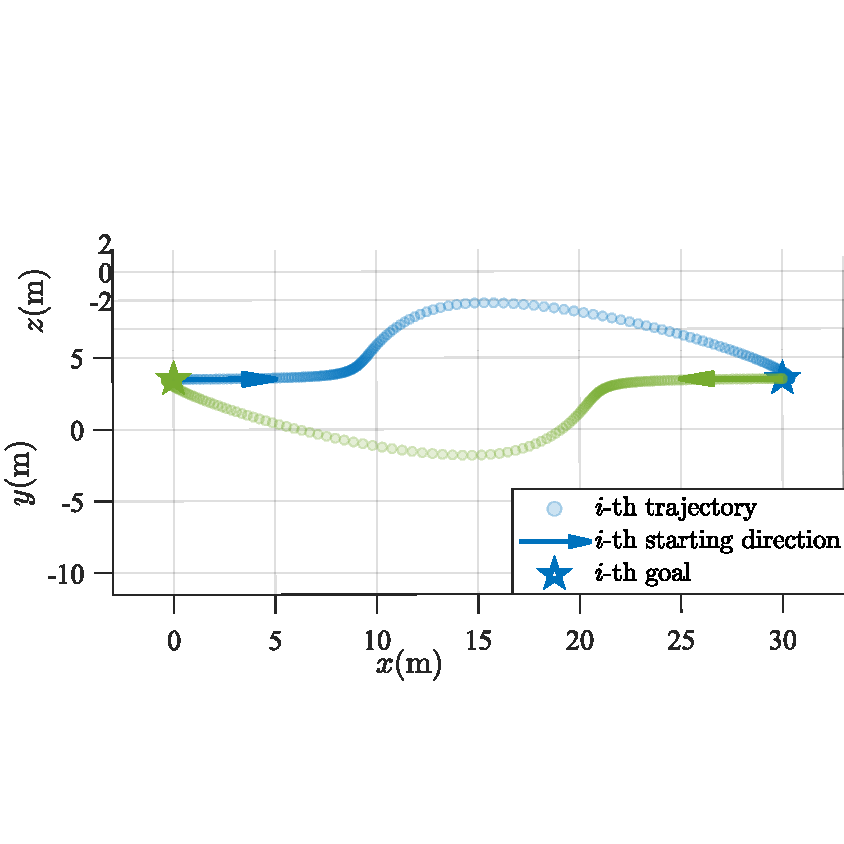
\includegraphics[width=0.31\linewidth, trim = \leftClip{} \lowerClip{} \rightClip{} \upperClip{}]{priv1.pdf} \label{fig:priv1}} \hfil
   \subfloat[$p_{12} = 0.7, p_{21} = 0.3$]{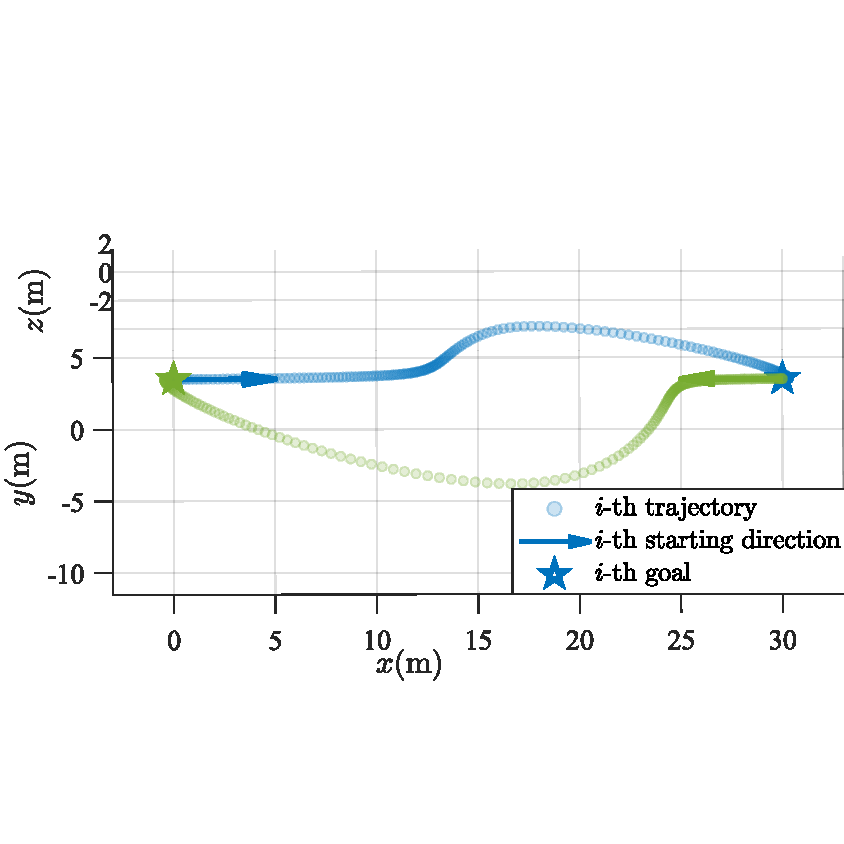
\includegraphics[width=0.31\linewidth, trim = \leftClip{} \lowerClip{} \rightClip{} \upperClip{}]{priv2.pdf} \label{fig:priv2} } \hfil
   \subfloat[$p_{12} = 1.0, p_{21} = 0.0$]{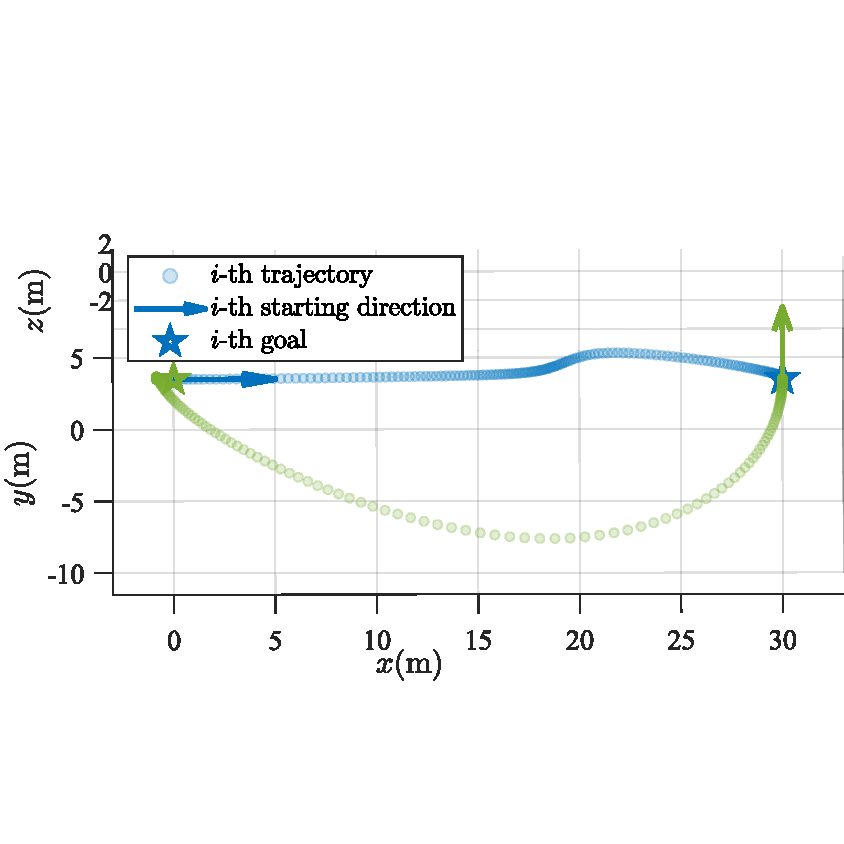
\includegraphics[width=0.31\linewidth, trim = \leftClip{} \lowerClip{} \rightClip{} \upperClip{}]{priv3.pdf} \label{fig:priv3} }
   \caption{Agents' behavior with different priority parameters.}
   \label{fig:priorityIllustration}
 \end{figure*}

\par The following result renders that two satellites are collision-free if both of the them follow the ``safety protocol''.

\begin{thm} \label{thm:safeProtocol}
   For systems discribed as (\ref{eqn:dynamics1}) and (\ref{eqn:dynamics2}), $\mathfrak{S}_{0ij}$ is forward invariant if $\boldsymbol{u}_i \in \mathcal{S}_{ij}, \boldsymbol{u}_j \in \mathcal{S}_{ji}$ and $p_{ij} + p_{ji} \le 1$.
\end{thm}

\begin{pf}
The proof mainly leverages Theorem \ref{thm:HOCBF}.
Let
\begin{equation}
    h_{ij} = d_{ij} - R_{ij} = \Psi_{0ij}
\end{equation}
be the HOCBF candidate to keep agent $i$ and agent $j$ collision-free.
By choosing positive proportional functions as class $\mathcal{K}_{\infty}$ functions, it follows the definition that
\begin{equation}
\begin{aligned}
      \Psi_{1ij} =& \dot{\Psi}_{0ij} + \alpha_1 (\Psi_{0ij}) \\
                 =& \frac{\boldsymbol{p}_i^{\top} - \boldsymbol{p}_j^\top}{d_{ij}} (\boldsymbol{v}_1 - \boldsymbol{v}_2) + \alpha_1 (d_{ij} - R_{ij}) \\
                 =&  \hat{\boldsymbol{n}}_{ij}^\top \boldsymbol{v}_{ij} + \alpha_1 \cdot \Psi_{0ij}.
\end{aligned}
\end{equation}
To get the constraint on control, we further define
\begin{equation} \label{eqn:psiDefinition}
   \begin{aligned}
      \Psi_{2ij} =& \dot{\Psi}_{1ij} + \alpha_2 \Psi_{1ij} \\
                 =& \frac{1}{d_{ij}^2}\left( (\boldsymbol{v}_i - \boldsymbol{v}_j)^{\top}d_{ij} - (\hat{\boldsymbol{n}}_{ij}^\top \boldsymbol{v}_{ij})(\boldsymbol{p}_i - \boldsymbol{p}_j)^{\top} \right) \boldsymbol{v}_{ij} \\
                 &+ \hat{\boldsymbol{n}}_{ij}^\top (\boldsymbol{u}_i + \boldsymbol{f}_{vi} - \boldsymbol{u}_j - \boldsymbol{f}_{vj}) + \alpha_1 \hat{\boldsymbol{n}}_{ij}^\top \boldsymbol{v}_{ij} \\
                 &+ \alpha_2 (\hat{\boldsymbol{n}}_{ij}^\top \boldsymbol{v}_{ij} + \alpha_1 \Psi_{0ij}) \\
                 =& \hat{\boldsymbol{n}}_{ij}^\top \left(\boldsymbol{u}_i - \boldsymbol{u}_j + (\alpha_1 + \alpha_2)\boldsymbol{v}_{ij} + \boldsymbol{f}_{vi} - \boldsymbol{f}_{vj} \right) \\
                 &+ \frac{1}{d_{ij}} \left( \|\boldsymbol{v}_{ij}\|^2 -  (\hat{\boldsymbol{n}}_{ij}^{\top}\boldsymbol{v}_{ij} )^2 \right) + \alpha_1 \alpha_2 (d_{ij} - R_{ij})
   \end{aligned}
\end{equation}
Given that $\boldsymbol{u}_i \in \mathcal{S}_{ij}$ and $\boldsymbol{u}_j \in \mathcal{S}_{ji}$, by adding up the inequalities in the definition of $\mathcal{S}_{ij}$ and $\mathcal{S}_{ji}$ and substituting $\hat{\boldsymbol{n}}_{ji} = -\hat{\boldsymbol{n}}_{ij}$ into the inequality, one can get
\begin{equation}
   \begin{aligned}
      \tilde{\Psi}_{2ij} =& \hat{\boldsymbol{n}}_{ij}^\top \left(\boldsymbol{u}_i - \boldsymbol{u}_j + (\alpha_1 + \alpha_2)\boldsymbol{v}_{ij} + \boldsymbol{f}_{vi} - \boldsymbol{f}_{vj} \right) \\
      &+ (p_{ij} + p_{ji})\left[ \frac{1}{d_{ij}} \left( \|\boldsymbol{v}_{ij}\|^2 -  (\hat{\boldsymbol{n}}_{ij}^{\top}\boldsymbol{v}_{ij} )^2 \right) \right. \\
      &+ \left. \alpha_1 \alpha_2 (d_{ij} - R_{ij}) 
            \vphantom{ \frac{1}{d_{ij}} \left( \|\boldsymbol{v}_{ij}\|^2 -  (\hat{\boldsymbol{n}}_{ij}^{\top}\boldsymbol{v}_{ij} )^2 \right) } 
         \right] \ge 0
   \end{aligned}
\end{equation}
Notice that $\|\boldsymbol{v}_{ij}\|^2 -  (\hat{\boldsymbol{n}}_{ij}^{\top}\boldsymbol{v}_{ij} )^2  \ge 0$ and $d_{ij} - R_{ij} \ge 0$ hold for $\left( \boldsymbol{x}_i(0), \boldsymbol{x}_j(0) \right) \in \mathfrak{S}_{0ij}$, $\Psi_{2ij} \ge \tilde{\Psi}_{2ij} \ge 0$ then stands for any $p_{ij}$ and $p_{ji}$ satisfying $p_{ij} + p_{ji} \le 1$.
Consequently, according to Definition \ref{def:HOCBF} and Theorem \ref{thm:HOCBF}, $h_{ij}$ is a valid HOCBF and thus $\mathfrak{S}_{0ij}$ is a forward invariant set for agent $i$ and agent $j$.
\end{pf}

Based on the properties of ``safe protocol'' set, we further design the distributed safeguarding policy in a minimum invasive way as
\begin{equation}\label{eqn:strategy}
   \boldsymbol{\pi}_i(\boldsymbol{u}_{ri}, \boldsymbol{X}) = 
   \left\{
   \begin{aligned}
      &\mathop{\arg \min}_{\boldsymbol{u} \in \cap_{j \neq i} \mathcal{S}_{ij}} \| \boldsymbol{u} - \boldsymbol{u}_{ri} \|^2,    &\cap_{j \neq i} \mathcal{S}_{ij} \neq \varnothing, \\
      &\mathop{\arg \min}_{\boldsymbol{u} \in \mathbb{R}^3 }\mathop{\max}_{j \neq i} \mathop{\mathrm{ESDF}}(\boldsymbol{u}, \mathcal{S}_{ij}),     &\cap_{j \neq i} \mathcal{S}_{ij} = \varnothing,
   \end{aligned}
   \right.
\end{equation}
where $\mathop{\mathrm{ESDF}}(\boldsymbol{u}, \mathcal{S}_{ij})$ is the Euclidean signed distance function (ESDF) of $\boldsymbol{u}$ to the boundary of half-space $\mathcal{S}_{ij}$, with $\mathop{\mathrm{ESDF}}(\boldsymbol{u}, \mathcal{S}_{ij})$ defined to be negative if $\boldsymbol{u} \in \mathcal{S}_{ij}$.

\par If $\cap_{j\neq i} \mathcal{S}_{ij} \neq \varnothing$, $\boldsymbol{\pi}_i$ minimally modifies $\boldsymbol{u}_{ri}$ to follow all ``safety protocols''.And $\boldsymbol{\pi}_i$ is now in the form of a quadratic programming and can be solved in real time onboard \cite[]{Ames2019CBFreview}; 
If $\cap_{j\neq i} \mathcal{S}_{ij} = \varnothing$, it is then impossible for agent $i$ to follow all ``safety protocols''. Therefore, $\boldsymbol{\pi}_i$ synthesises a control that minimizes the maximum violation of all ``safe protocols'' to get the ``safest possible'' control.
Such an optimization can also be solved in real time onboard via a linear programming \cite[]{Berg2011ORCA}.

\begin{thm}
   If $\cap_{j\neq i} \mathcal{S}_{ij} \neq \varnothing$ for all agent $i$, $\mathfrak{S}_0$ is forward invariant if $\boldsymbol{u}_i = \boldsymbol{\pi}_i(\boldsymbol{u}_{ri}, \boldsymbol{X})$ and $\boldsymbol{P} = \{p_{ij}\}_{(N\times N)} \in \left\{ \boldsymbol{P} \in \mathbb{R}^{N\times N} \mid p_{ii} = 0,  p_{ij} + p_{ji} \le 1, i\neq j \right\}$.
\end{thm}
\begin{pf}
   This result directly follows Theorem \ref{thm:safeProtocol}. 
   Given that $\cap_{j\neq i} \mathcal{S}_{ij} \neq \varnothing, \forall i = 1, 
   \dots, N$, it cleary renders that $\boldsymbol{u}_i = \boldsymbol{\pi}_i(\boldsymbol{u}_{ri}, \boldsymbol{X}) \in \cap_{j\neq i} \mathcal{S}_{ij}$ is satisfied for all agents.
   Since for any satellite pair composed of satellite $i$ and satellite $j$, $\boldsymbol{u}_i \in \cap_{j\neq i} \mathcal{S}_{ij} \subseteq  \mathcal{S}_{ij}, \boldsymbol{u}_j \in \cap_{i\neq j} \mathcal{S}_{ji} \subseteq  \mathcal{S}_{ji}$ and $p_{ij} + p_{ji} \le 1$ are satisfied, according to Theorem \ref{thm:safeProtocol}, all $\mathfrak{S}_{0ij}, i \neq j$ are forward invariant.
   Hence their intersection $\mathfrak{S}_0 = \bigcap_{i \neq j}\mathfrak{S}_{0ij}, ~i,j = 1, \dots, N$ is forward invariant, rendering that the whole satellite swarm is collision-free.
\end{pf}

\begin{remark}
   The priority parameter $p_{ij}$ has a clear physical interpretation.
   Since $\|\boldsymbol{v}_{ij}\|^2 -  (\hat{\boldsymbol{n}}_{ij}^{\top}\boldsymbol{v}_{ij} )^2  \ge 0$ holds universally and $d_{ij} - R_{ij} \ge 0$ if agent $i$ and agent $j$ remain collision-free, the right hand side of (\ref{eqn:safeProtocol}) is monotonically increasing with $p_{ij}$.
   Consequently, higher $p_{ij}$ lowers the control modification required by agent $i$ to satisfy $\boldsymbol{u}_i \in \mathcal{S}_{ij}$.
   Given the constraint that $p_{ij} + p_{ji} \le 1$, this leads $p_{ij}$ to a decrease, causing agent $j$ to assume greater responsibility for avoiding collision with agent $i$.
   By tuning the priority matrix $\boldsymbol{P}$, high-level decisions can explicitly determine relative collision evasion responsibilities of satellites.
   Figure \ref{fig:priorityIllustration} illustrates  such a behavior: two identical satellites switching positions are simulated with varying $p_{ij}$.
   By increasing $p_{12}$ while decreasing $p_{21}$, satellite 1 (colored in blue) executes less evasive maneuvering, while satellite 2 (colored in red) executes more.
\end{remark}

\section{Cooperating with high-level decisions}\label{sec:decision}
\subsection{Cooperating with Optimization}
\par Centralized control struggles to meet high-frequency control demands for collision avoidance due to communication delays and computational burden.
Nevertheless, it can generate global reference behaviors that guide the distributed safety filter by optimizing the priority matrix.
With $\boldsymbol{u}_{ri}$ and $\boldsymbol{X}$ fixed, $\boldsymbol{\pi}_i$ depends only on $p_{ij}$ (i.e., $\boldsymbol{\pi}_i = \boldsymbol{\pi}_i (\boldsymbol{P})$). Thus, the priority matrix can be optimized to minimize the deviation of $\boldsymbol{U} = [\boldsymbol{u}_1^\top~\dots~\boldsymbol{u}_N^\top]^\top$ from $\boldsymbol{U}_{gr} = [\boldsymbol{u}_{gr1}^{\top}~\dots~\boldsymbol{u}_{grN}]^\top$ through
\begin{equation}\label{eqn:priorityOptimization}
\begin{aligned}
      & \boldsymbol{P}^{\ast} = \mathop{\arg \min}_{\boldsymbol{P} \in \mathbb{R}^{N\times N}} \| \boldsymbol{U}_{gr} - \boldsymbol{U}(\boldsymbol{P}) \|^2 \\
      \mathrm{s.t.}& \left\{ 
         \begin{aligned}
            &\boldsymbol{u}_i =  \boldsymbol{\pi}_i(\boldsymbol{P}), &\forall i = 1, \dots, N\\
            &p_{ij} + p_{ji} \le 1, &\forall i \neq j, i, j = 1, \dots, N\\
            &p_{ii} = 0, &\forall i = 1, \dots, N
         \end{aligned}   
      \right.
\end{aligned}
\end{equation}
By maximizing $p_{ij}$ to satisfy $p_{ij} + p_{ji} = 1$, optimization (\ref{eqn:priorityOptimization}) can thereby be reduced to an unconstrained problem: only the upper triangle elements $p_{ij}, i < j$ need optimization, with the lower triangle obtained through $p_{ji} = 1 - p_{ij}$.
This optimization extracts the assignment preferences of centralized control into $\boldsymbol{P}^{\ast}$, thereby coordinating the satellite swarm to align with global reference behaviors.

\subsection{Cooperating with Large Language Models}
\par While collision avoidance requirements are mathematically straightforward, mission-level objectives are significantly more complex and often specified in natural language. 
By leveraging the reasoning ability of LLMs, the aforementioned priority parameters can be generated according to the mission requirements, thereby allocating collision evasion responsibilities.

\par However, directly generate a priority matrix $\boldsymbol{P}$ satisfying $p_{ij} + p_{ji} \le 1, \forall i \neq j$ through LLM is challenging due to the black-box nature of LLMs.
As a result, instead of direct matrix generation, we use LLM to produce a priority array $\mathbf{p} = [p_1,~p_2,~\dots,~p_N], p_i \ge 0, \forall i = 1, \dots, N$, with $p_i$ representing the significance of satellite $i$ in the mission.
To ensure the output stability, structured output technique is adopted to force the output format on LLMs.
After getting the valid output, the priority parameters are calulated through $p_{ij} = p_i/(p_i + p_j)$ to inherently satisfy the safety condition.

\par Prompts are also carefully engineered to enhance LLM performance. A chain of thought is given to LLMs to first  classify satellites by role and mission priority levels, then assign base priorities according to levels, and finally adjust priorities for satellites within the same level.
Demonstrations are also provided to leverage the LLM's in-context learning capabilities \cite[]{Min2022fewshot}.

\begin{figure*}[t!]
   \newcommand{\upperClip}{0bp}
   \newcommand{\lowerClip}{0bp}
   \newcommand{\leftClip}{0bp}
   \newcommand{\rightClip}{0bp}
   \centering
   \subfloat[Fixed priority]{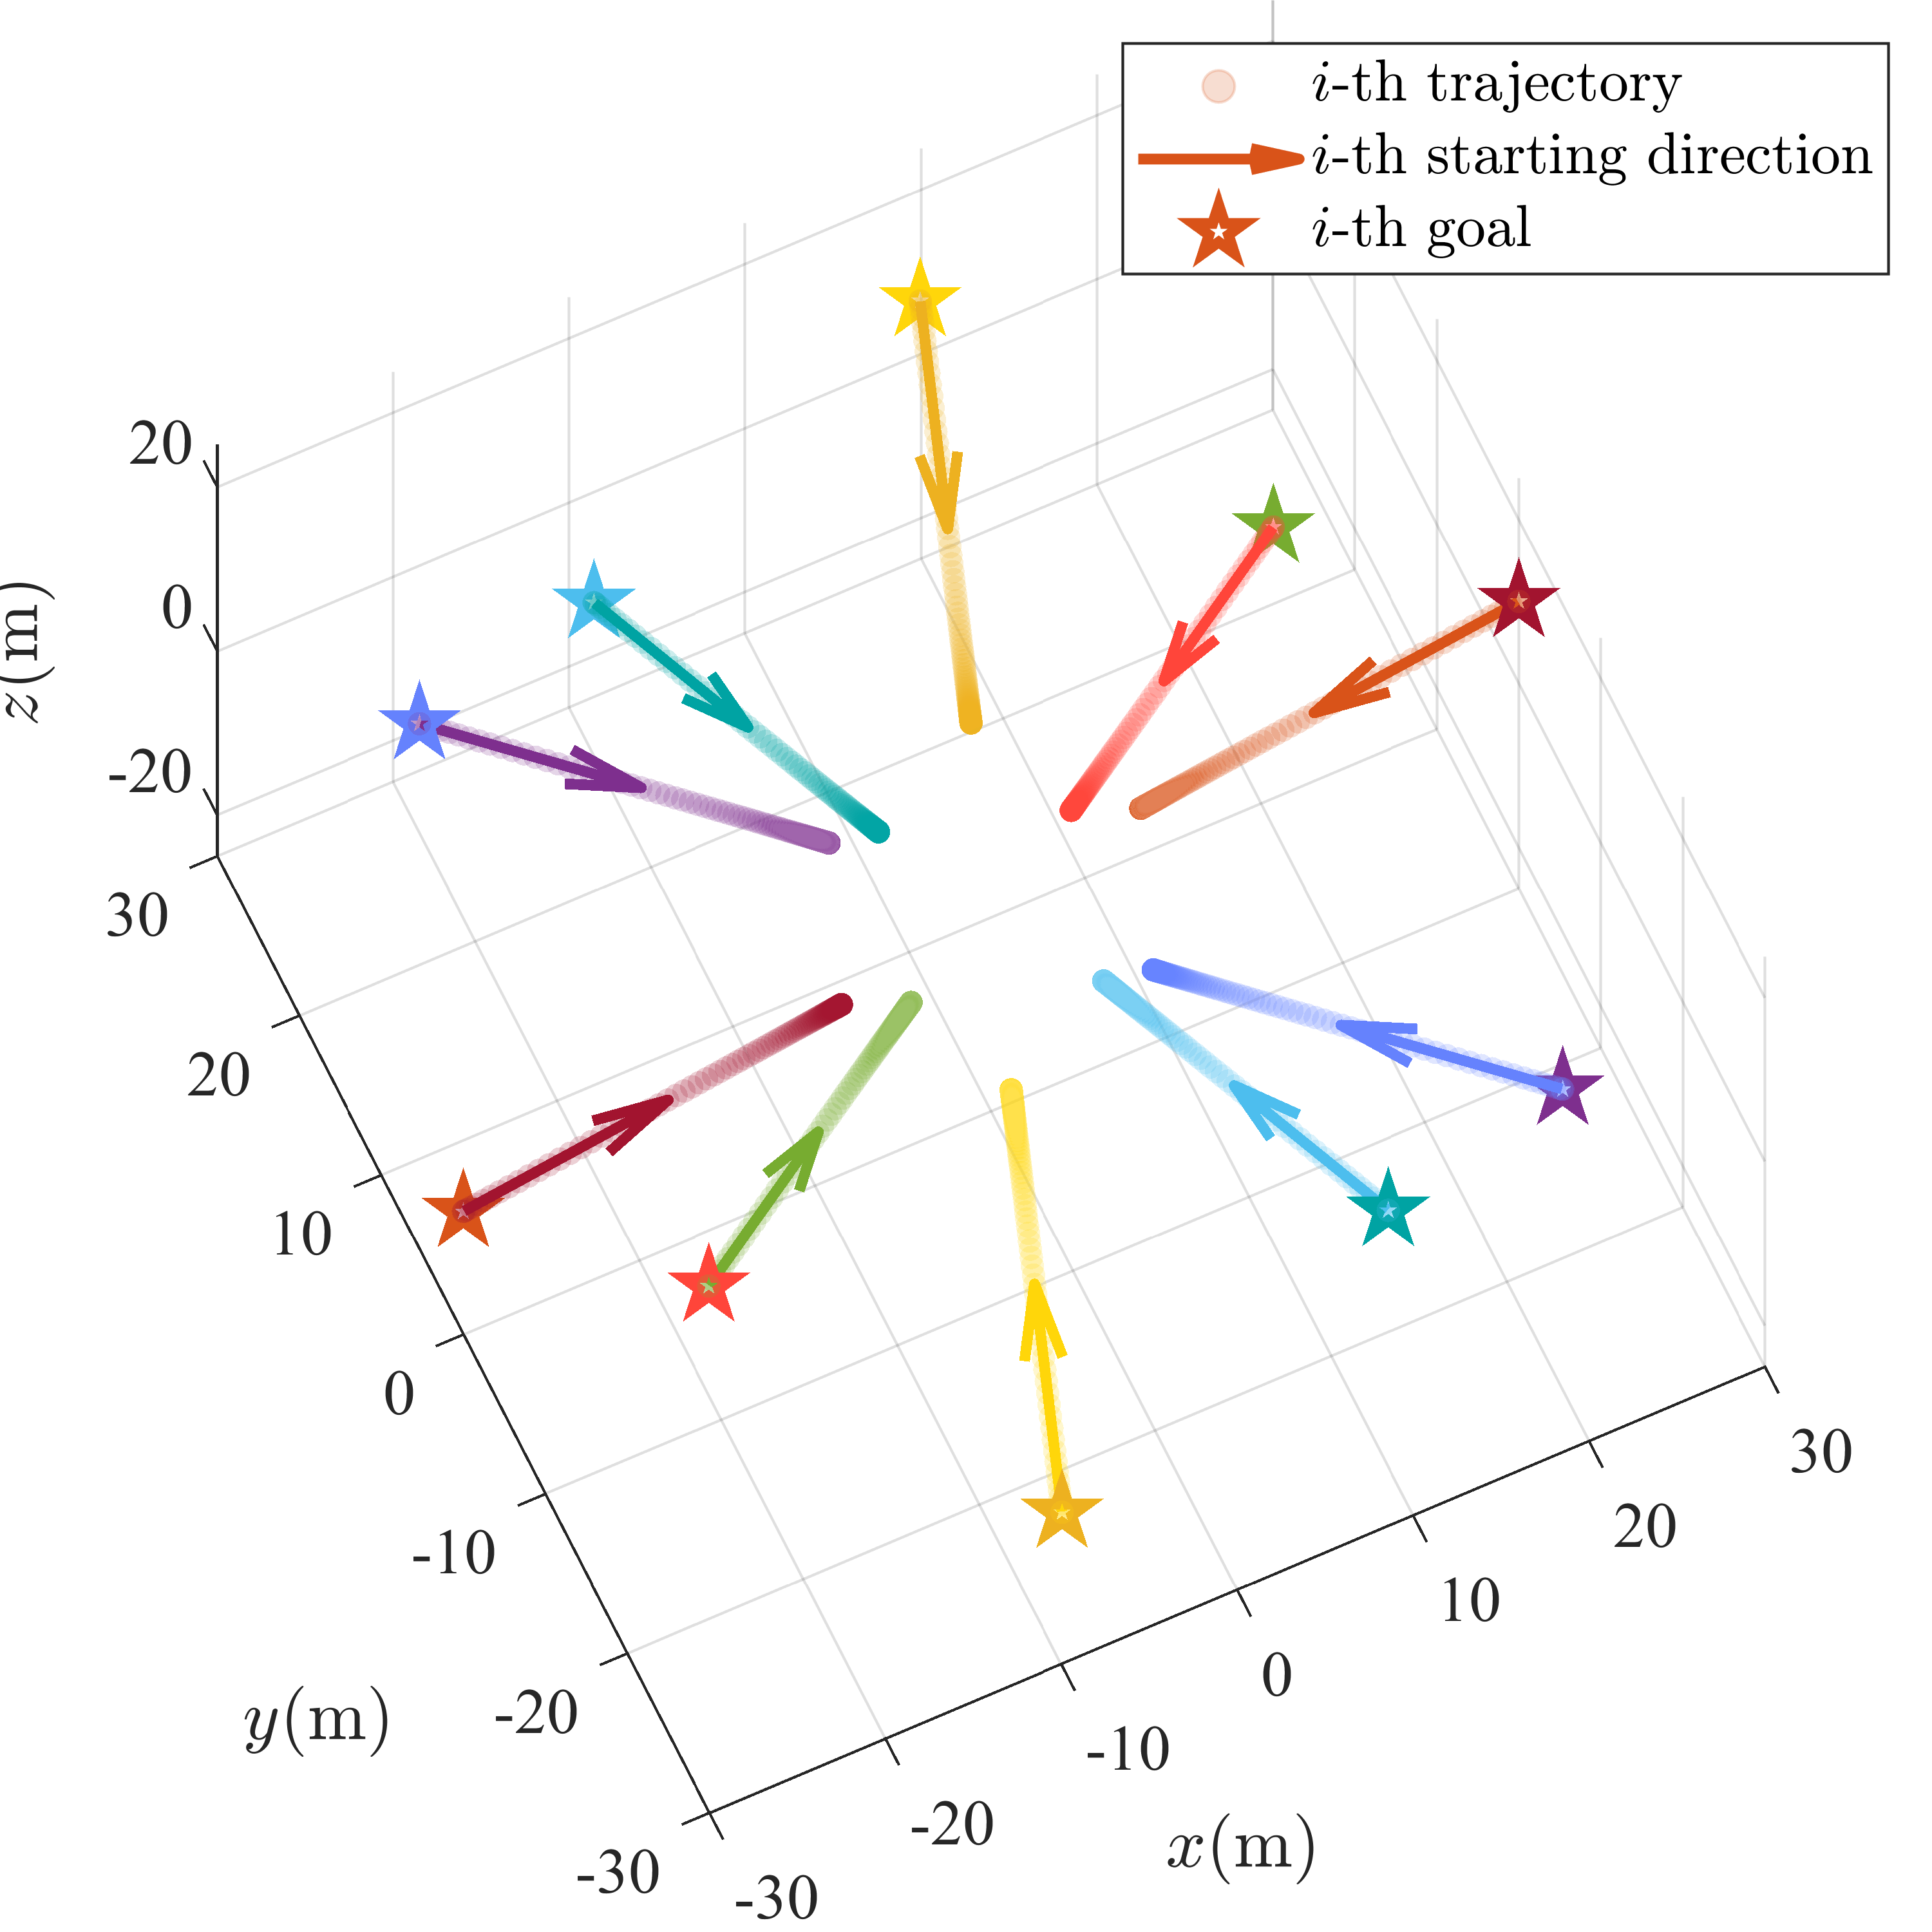
\includegraphics[width=0.45\linewidth, trim = \leftClip{} \lowerClip{} \rightClip{} \upperClip{}, clip]{opt1.png} \label{fig:opt1}} \hfil
   \subfloat[Centralized control]{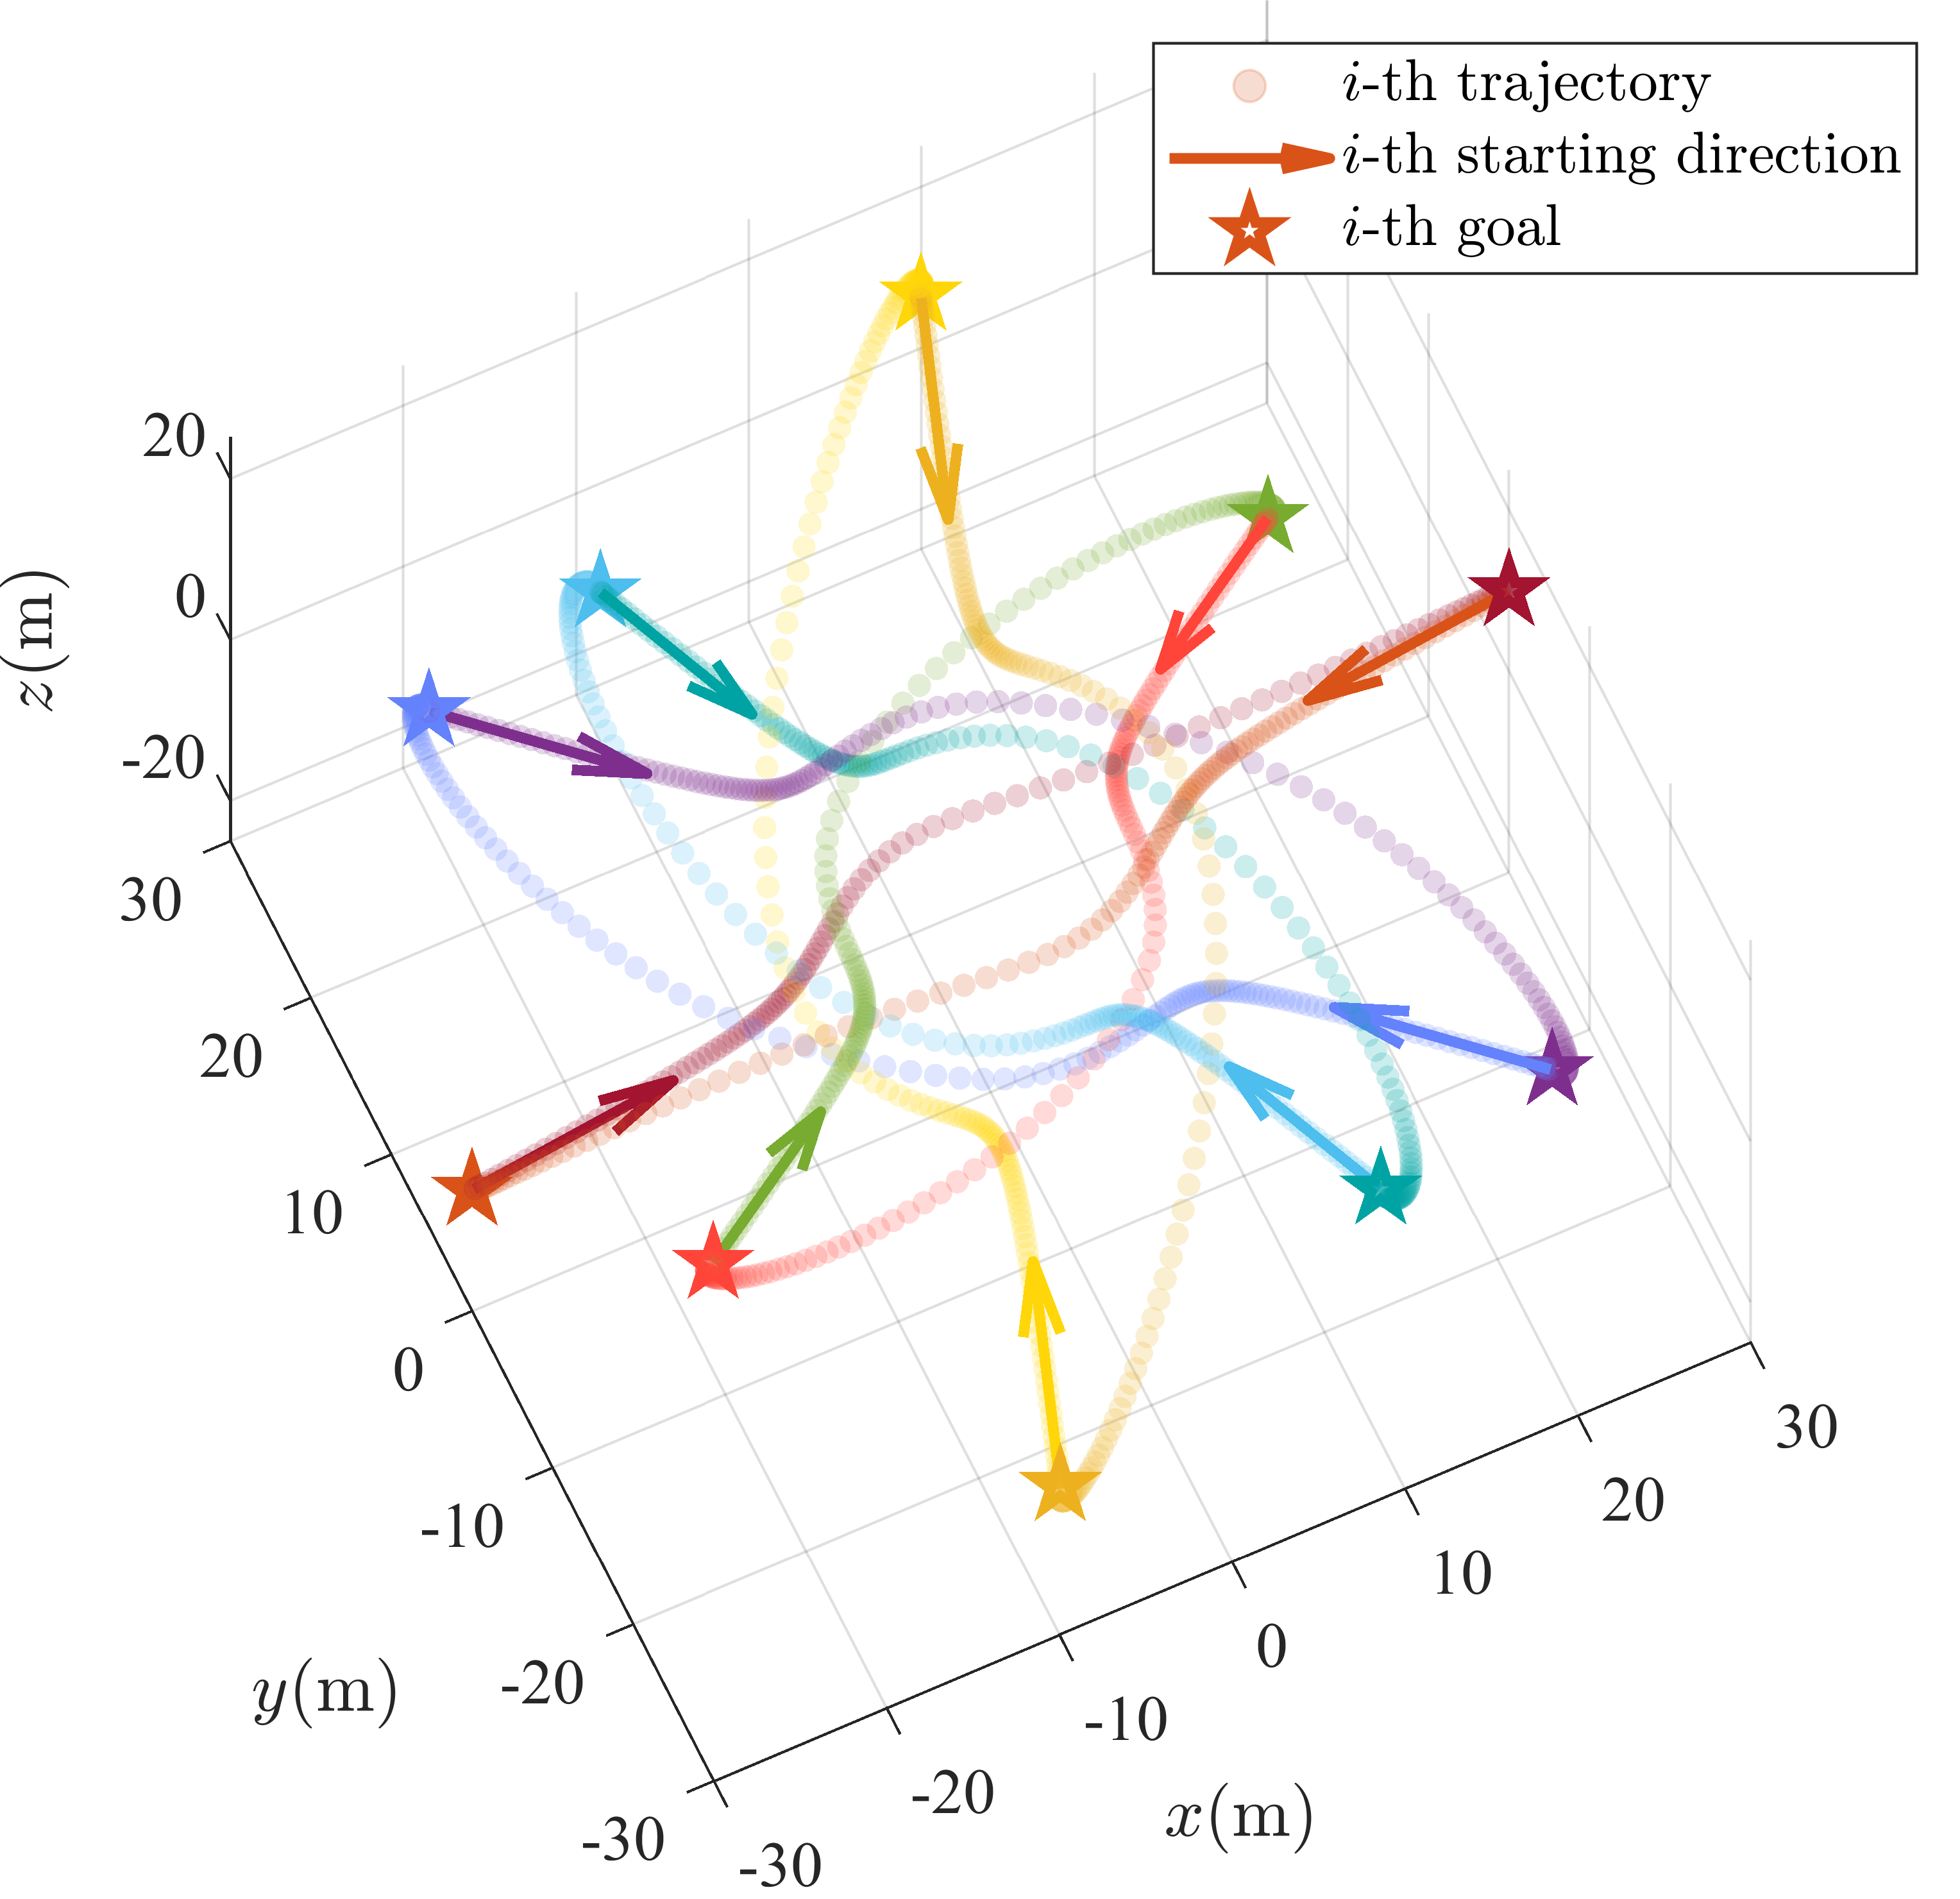
\includegraphics[width=0.45\linewidth, trim = \leftClip{} \lowerClip{} \rightClip{} \upperClip{}, clip]{opt2.png} \label{fig:opt2} } \\
   \subfloat[Optimized priority]{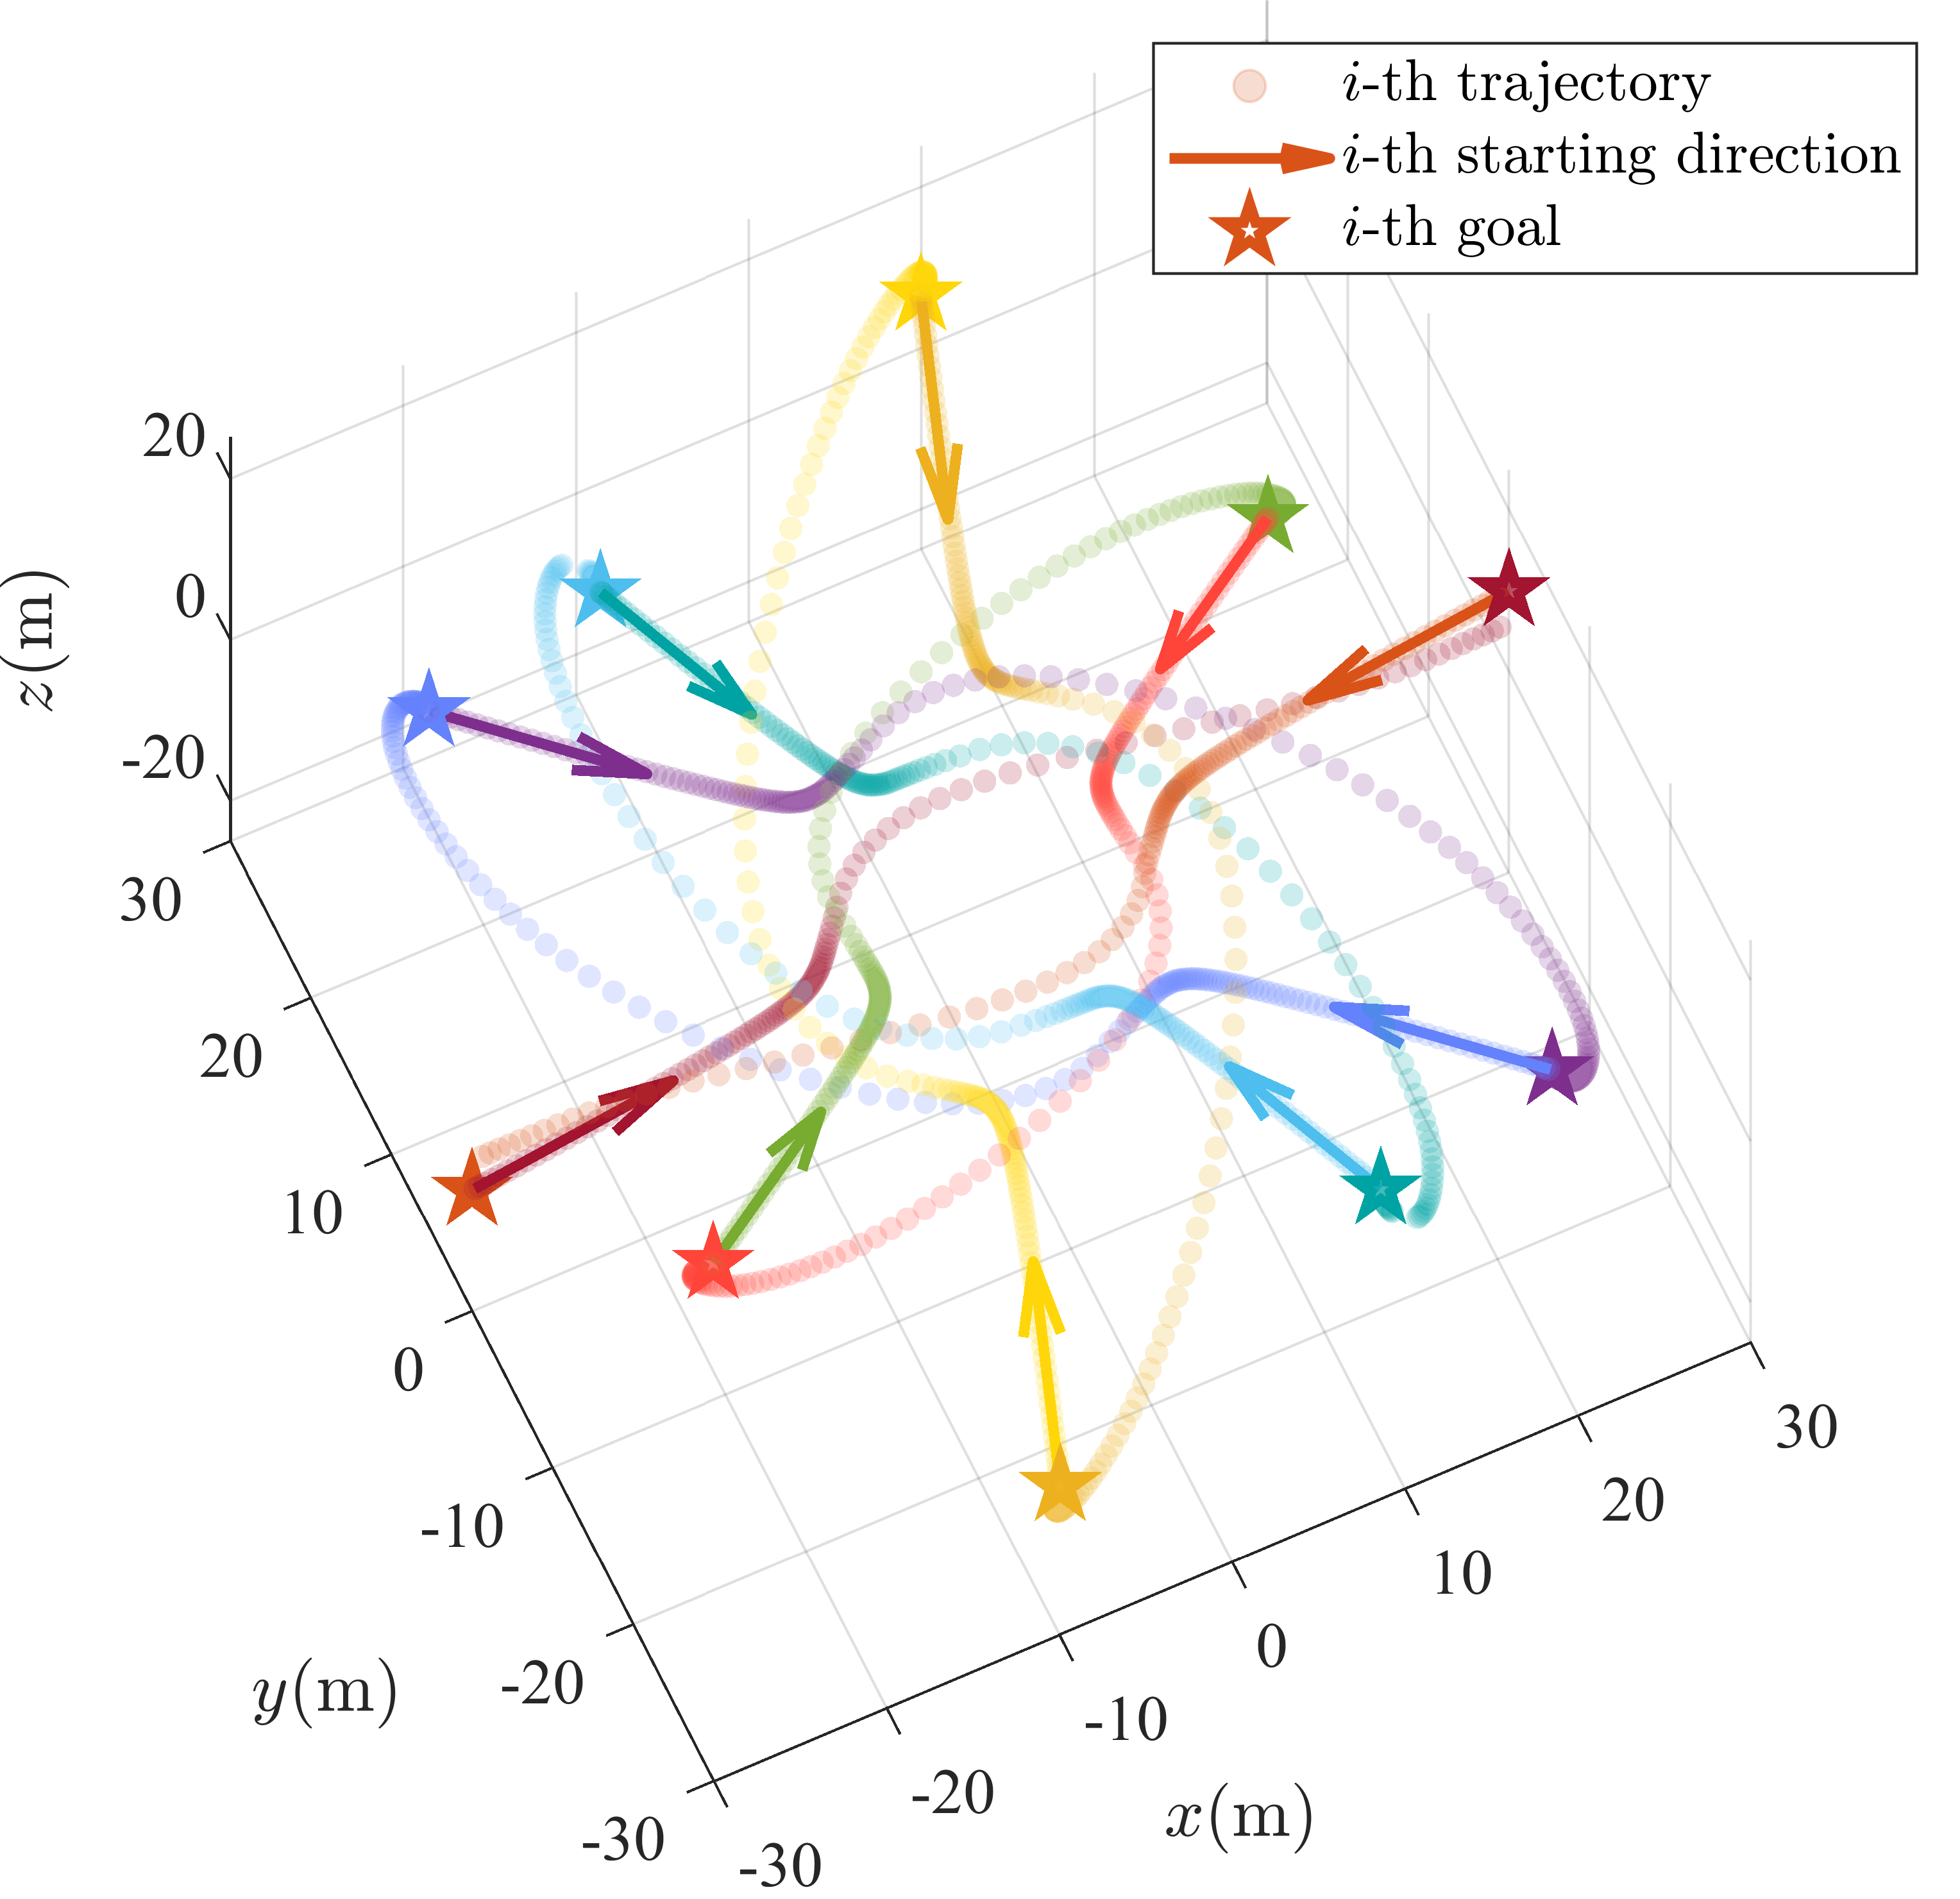
\includegraphics[width=0.45\linewidth, trim = \leftClip{} \lowerClip{} \rightClip{} \upperClip{}, clip]{opt3.png} \label{fig:opt3} } \hfil
   \subfloat[Non-cooperative]{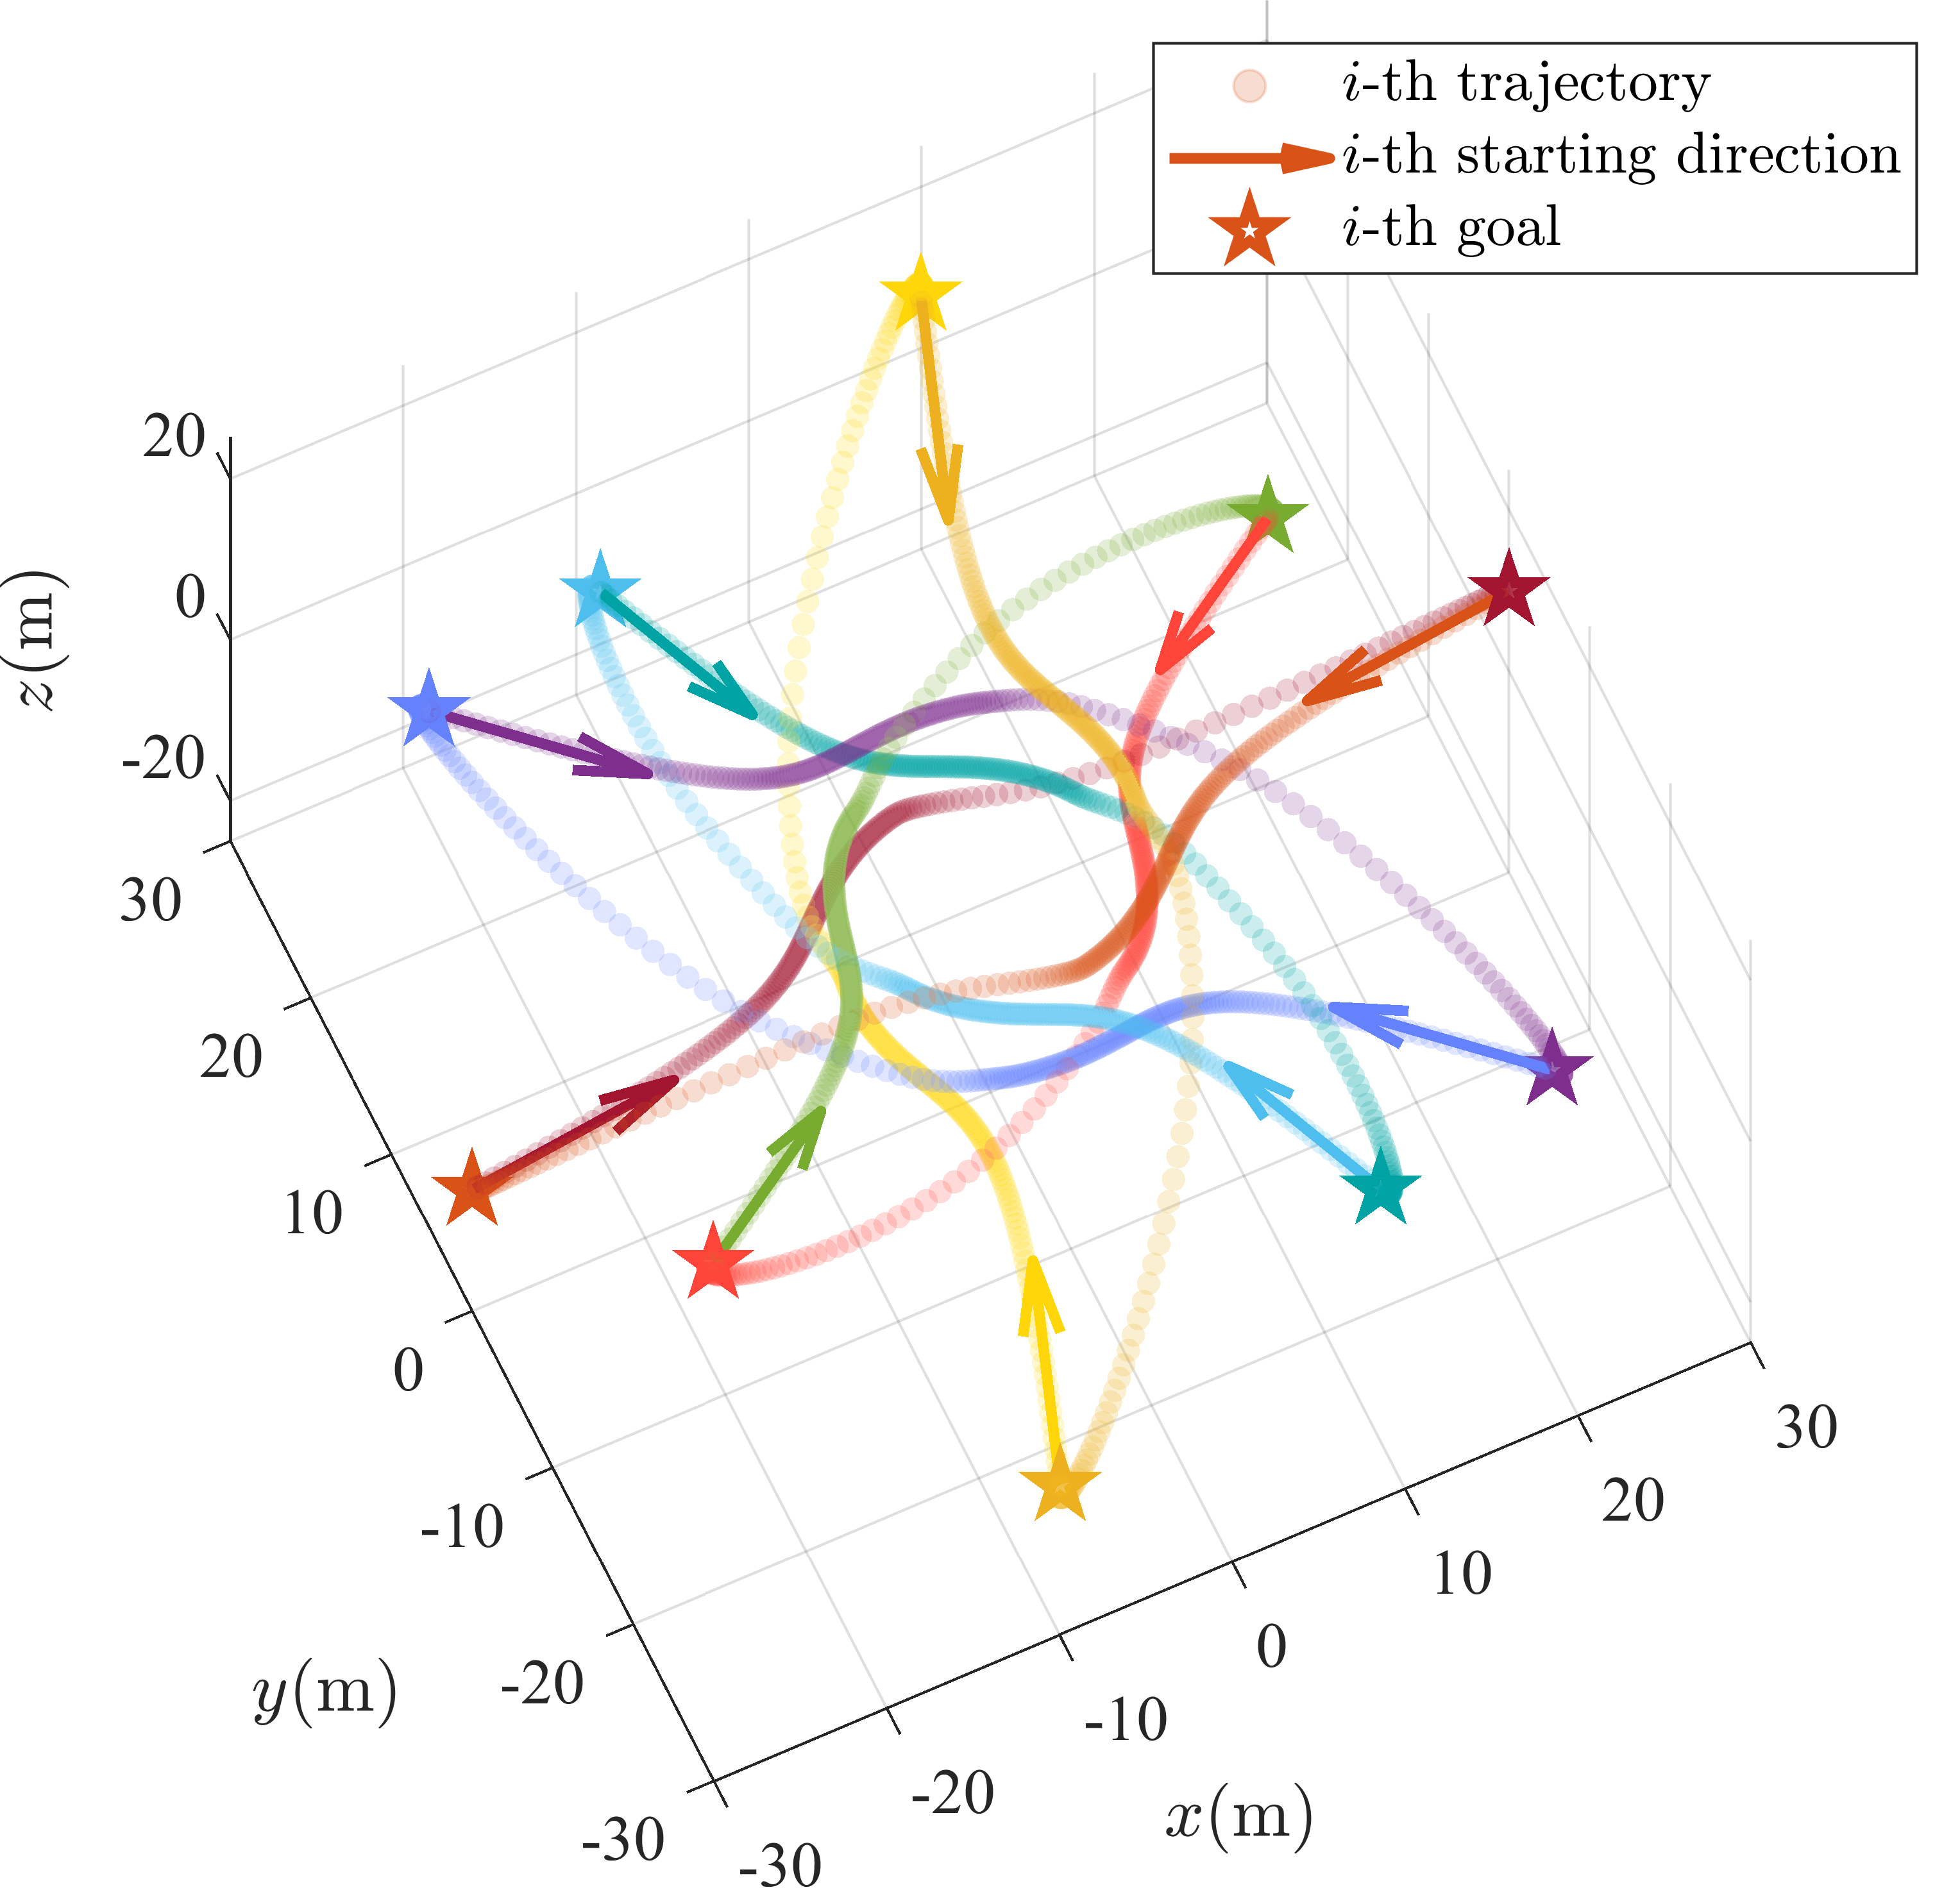
\includegraphics[width=0.45\linewidth, trim = \leftClip{} \lowerClip{} \rightClip{} \upperClip{}, clip]{opt4.png} \label{fig:opt4}} 
   \caption{Swarm behavior with different collision avoidance strategies.}
   \label{fig:optexp}
\end{figure*}

\section{Numerical Simulations}\label{sec:exp}
% \par We validate the efficacy of the distributed safety filter by cooperating with optimization and LLM, respectively. 
% In the experiments, the safety distance of each agent is set to $r_i = 5\mathrm{m}, i = 1, \dots, N$ and $\omega$ is set to $0.00113 \mathrm{rad/s}$, which is approximatly the angular velocity of International Space Station.

\subsection{Cooperating with Optimization}
\par We demonstrate the proposed method by comparing four approaches: fixed priority, centralized control, optimized priority (proposed), and non-cooperative.
For the first case, the control of each agent is calculated distributedly by (\ref{eqn:strategy}) with $p_{ij} = 0.5, \forall i \neq j$.
For the centralized control case, the control is calculated centrally through 
\begin{equation}\label{eqn:centralizedStrategy}
\begin{aligned}
      &\boldsymbol{U} = \mathop{\arg \min}_{\boldsymbol{U}^{\prime} \in \mathbb{R}^{3 N}} \| \boldsymbol{U}^\prime - \boldsymbol{U}_r\|^2 \\
      &\mathrm{s.t.}  \Psi_{2ij} \ge 0, \forall i \neq j,
\end{aligned}
\end{equation}
where $\Psi_{2ij}$ is defined in (\ref{eqn:psiDefinition}) and $\boldsymbol{U}_r = [\boldsymbol{u}_{r1}^{\top}~\dots~\boldsymbol{u}_{rN}^{\top}]^\top$ denotes the reference control.
For the optimized priority case, control is calculated distributedly by (\ref{eqn:strategy}), with $\boldsymbol{P}$ centrally optimized every $10~\mathrm{s}$ using (\ref{eqn:priorityOptimization}) and $\boldsymbol{U}_{gr}$ derives from (\ref{eqn:centralizedStrategy}).
For the last case, control is calculated distributedly by each agent $i$ through
\begin{equation}
\begin{aligned}
      & \boldsymbol{u}_i = \mathop{\arg \min}_{\boldsymbol{u}_i^{\prime} \in \mathbb{R}^{3}} \| \boldsymbol{u}_i^\prime - \boldsymbol{u}_{ri}\|^2 \\
      & \mathrm{s.t.}  \Psi_{2ij} \ge 0, \forall i \neq j,
\end{aligned}
\end{equation}
with the assumption that $\boldsymbol{u}_j = \boldsymbol{0}, j \neq i$.  
All approaches above use $\boldsymbol{U}_r$ given by the same proportional derivative (PD) controller.

\par We evaluated all methods above on a position-swapping task where satellites move to their diametrically opposite positions. The trajectory of satellites is shown in {\figurename} \ref{fig:optexp} by plotting the position of each agent every $1.5~\mathrm{s}$. The starting directions of each satellite is illustrated by arrows, with the starting points of the arrows aligned with the initial positions of agents, and the directions of the arrows aligned with the velocity directions of each agent at $t = 0.5~\mathrm{s}$.
The minimum distance $h_{ij}$ appear in {\figurename} \ref{fig:minDistance}.

\par As shown in {\figurename} \ref{fig:opt1}, satellites encountered a deadlock in the first case, which is related to distributed and local design of the controller.
Since the centralized control case optimizes control globally, satellites were coordinated to their goals ({\figurename} \ref{fig:opt2}).
By using the centralized control above as a low frequency global reference, the proposed method avoided the deadlock as well with distributed control ({\figurename} \ref{fig:opt3}).
The non-cooperative case coordinated the satellites to their goals as well ({\figurename} \ref{fig:opt4}). 
However, as shown in {\figurename} \ref{fig:minDistance}, such a method appears to be invalid since collision occured between $150~\mathrm{s}$ and $200~\mathrm{s}$.
This happened due to invalid $\boldsymbol{u}_j = \boldsymbol{0}, j \neq i$ assumptions.
These results above demonstrate that our distributed safety filter can effectively leverage global reference behaviors through priority optimization.

\subsection{Cooperating with Large Language Models}
\par We further demonstrate the effectiveness of LLM integration with our safety filter. A local \texttt{Gemma3:12b} \cite[]{gemma2024} model is deployed to generate priority assignments for a 6-satellite position-swapping task under three distinct prompts. 
In the first case, LLM was informed that ``Satellite 1 is mission critical. All other satellites are backup satellites''; 
in the second, LLM was given the prompt that ``Satellite 1 is mission critical. All other satellites have low fuel'';
in the last case, LLM was hinted that ``All satellites are the same''.
The trajectories of satellite are shown in {\figurename} \ref{fig:llmexp}, with $T_1$ representing the time required by satellite 1 to arrive its goal.

\par Given the prompts above, LLM outputted the priority array as $\mathbf{p} = [10, 1, 1, 1, 1, 1]$, $\mathbf{p} = [9, 7, 7, 7, 7, 7]$ and $\mathbf{p} = [5, 5, 5, 5, 5, 5]$, respectively. 
Consequently, the priority parameter $p_{1j}, j\neq 1$ decreased progressively across cases.
The difference of $p_{1j}$ is then reflected on the trajectory and arriving time of satellite 1. 
From {\figurename} \ref{fig:llm1} to {\figurename} \ref{fig:llm3}, satellite 1 experienced increasing safety filter interventions, which in turn increased the curvature of the satellite 1's trajectory and therefore lengthened $T_1$ from $204.5~\mathrm{s}$ to $321.5~\mathrm{s}$.
This demonstrates our framework's capacity to adapt collision evasion responsibilities to mission requirements through LLM-generated priorities.

\begin{figure}[!t]
   \begin{center}
      \newcommand{\upperClip}{30bp}
      \newcommand{\lowerClip}{8bp}
      \newcommand{\leftClip}{10bp}
      \newcommand{\rightClip}{10bp}
      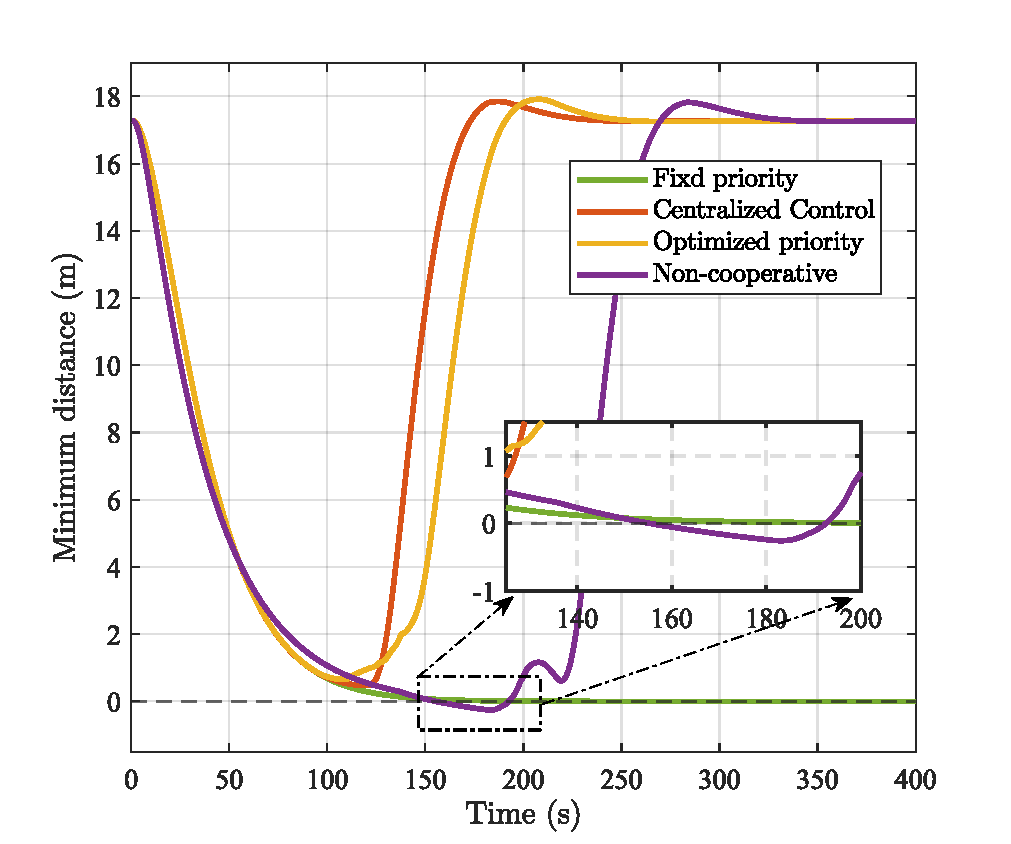
\includegraphics[width=1.0\linewidth, trim = \leftClip{} \lowerClip{} \rightClip{} \upperClip{}, clip]{minDistance.pdf} 
      \caption{Minimum distance between satellites with different collision avoidance strategies} 
      \label{fig:minDistance}
   \end{center}
\end{figure}

\begin{figure}[!t]
   \newcommand{\upperClip}{40bp}
   \newcommand{\lowerClip}{20bp}
   \newcommand{\leftClip}{0bp}
   \newcommand{\rightClip}{0bp}
   \centering
   \subfloat[$T_1 = 204.5\mathrm{s}$]{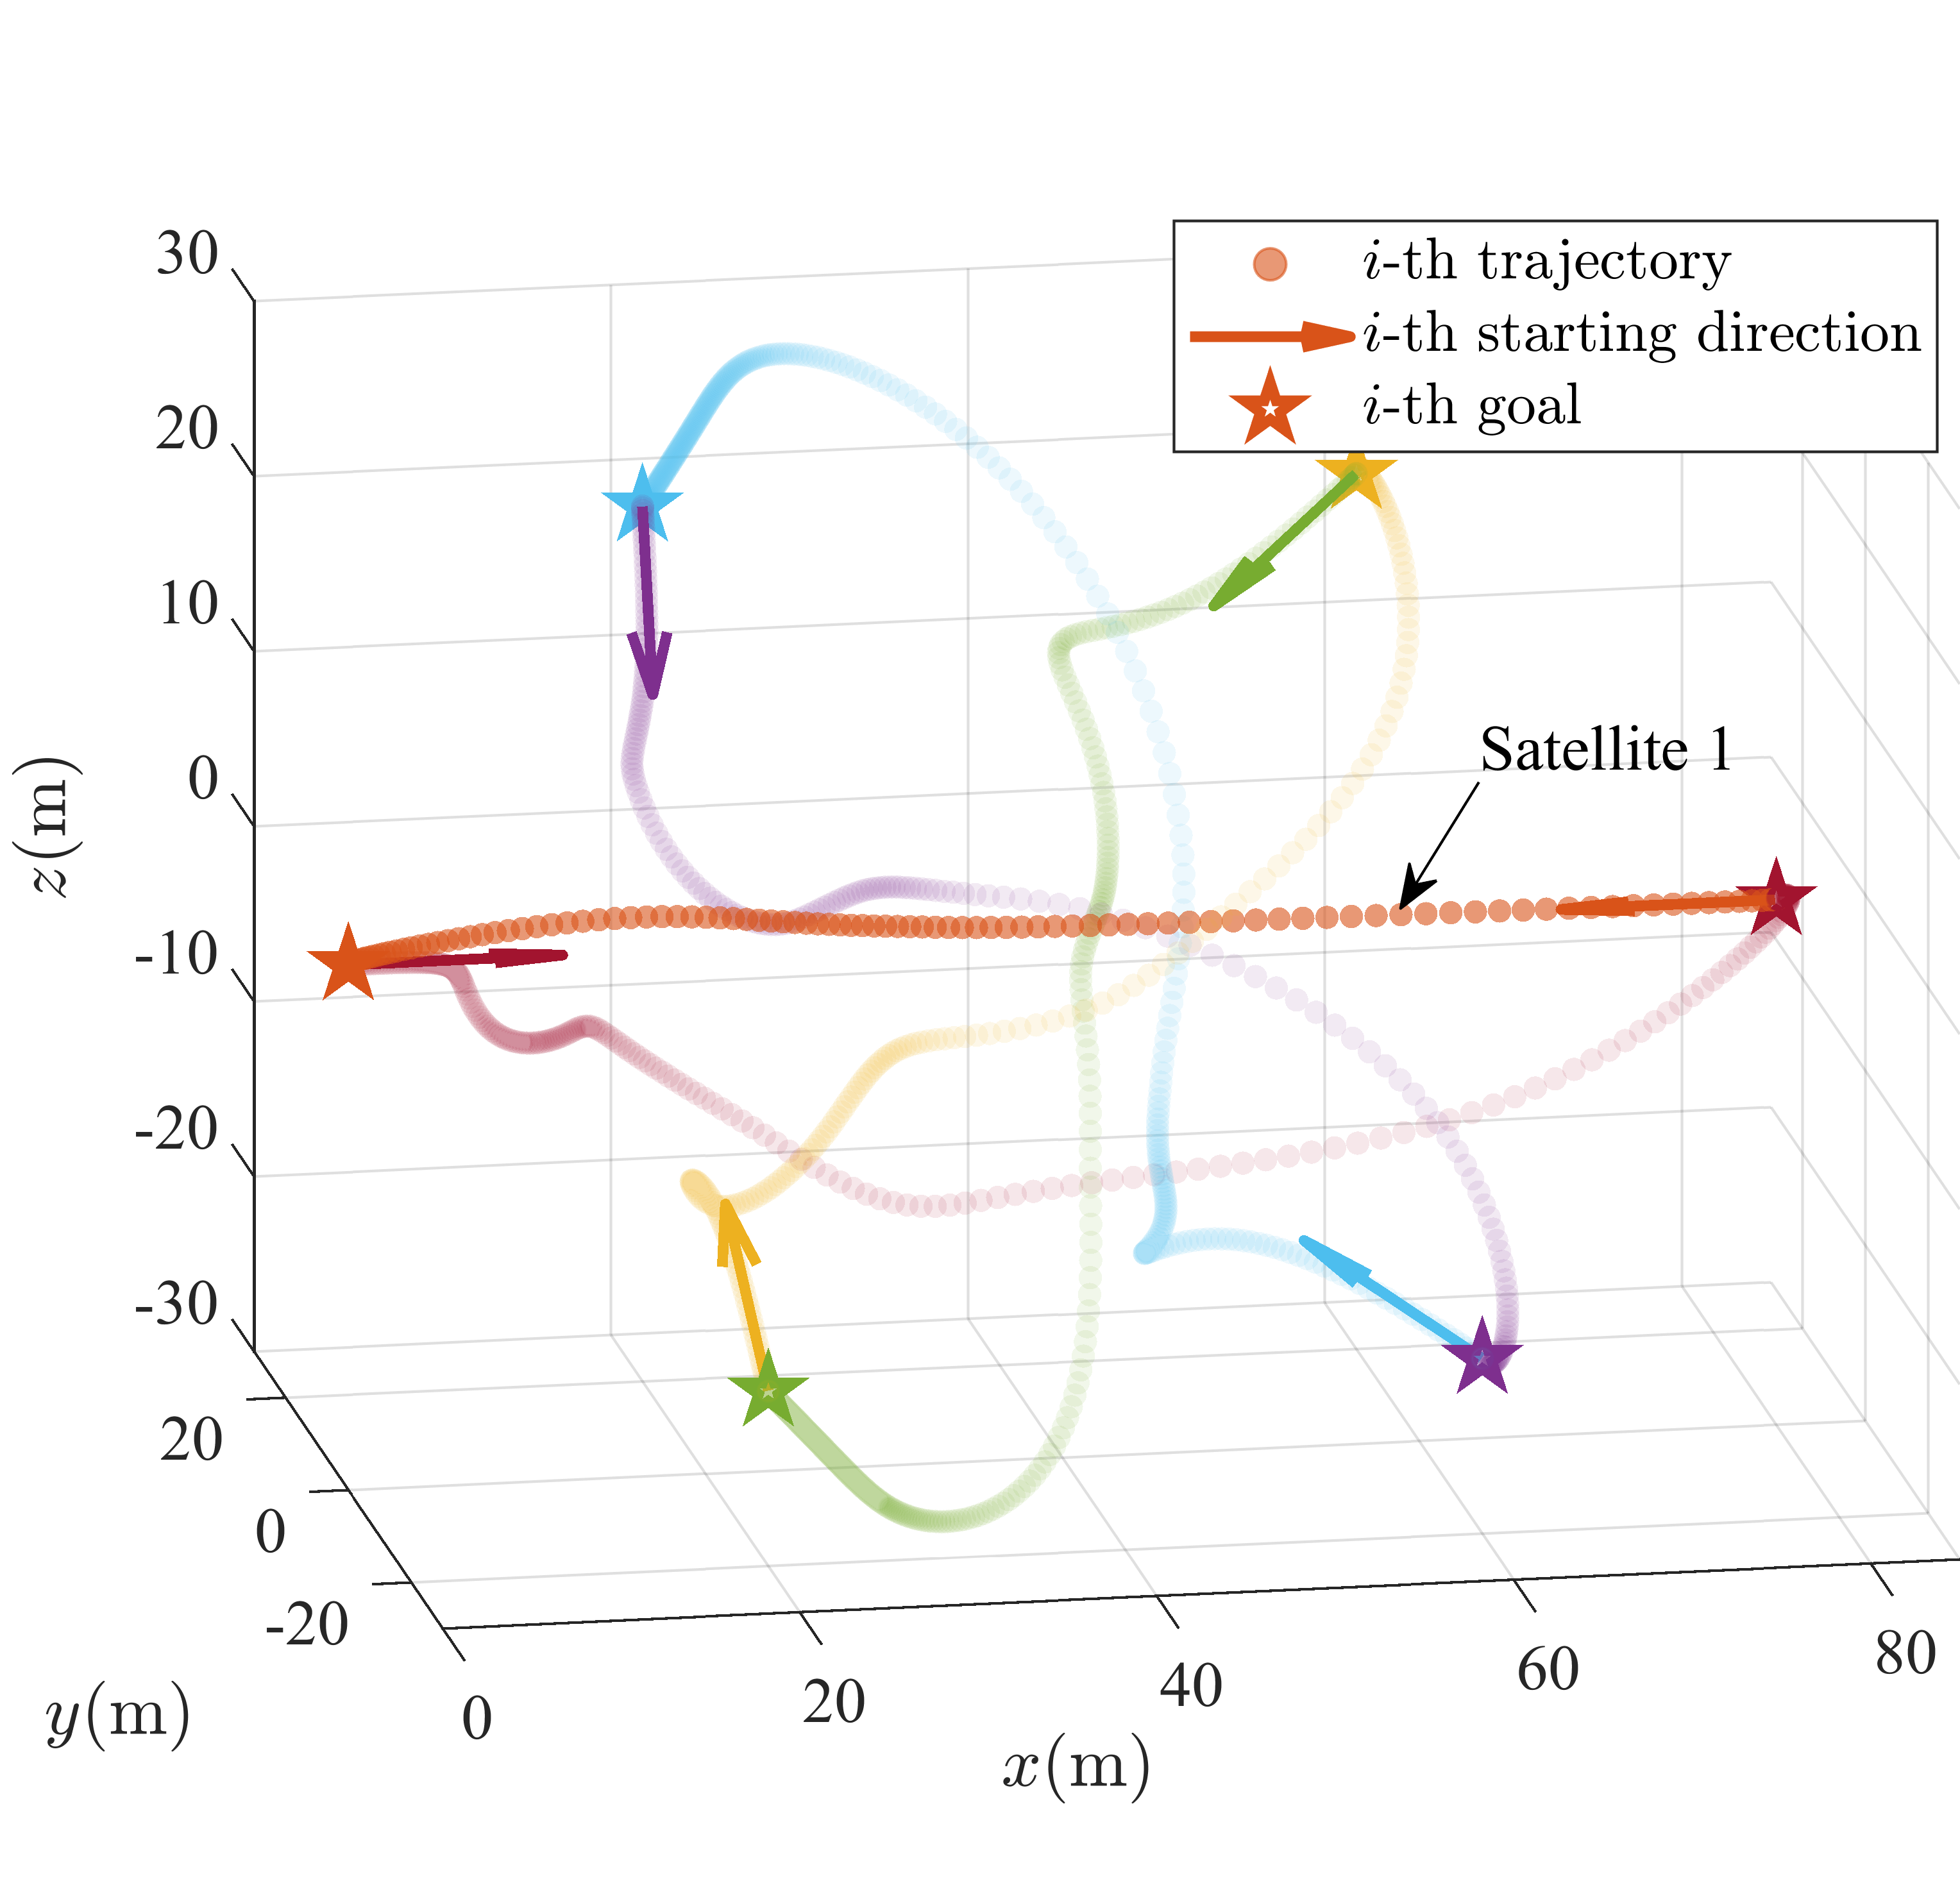
\includegraphics[width=0.9\linewidth, trim = \leftClip{} \lowerClip{} \rightClip{} \upperClip{}, clip]{llm1.png} \label{fig:llm1}} \\
   \subfloat[$T_1 = 295.5\mathrm{s}$]{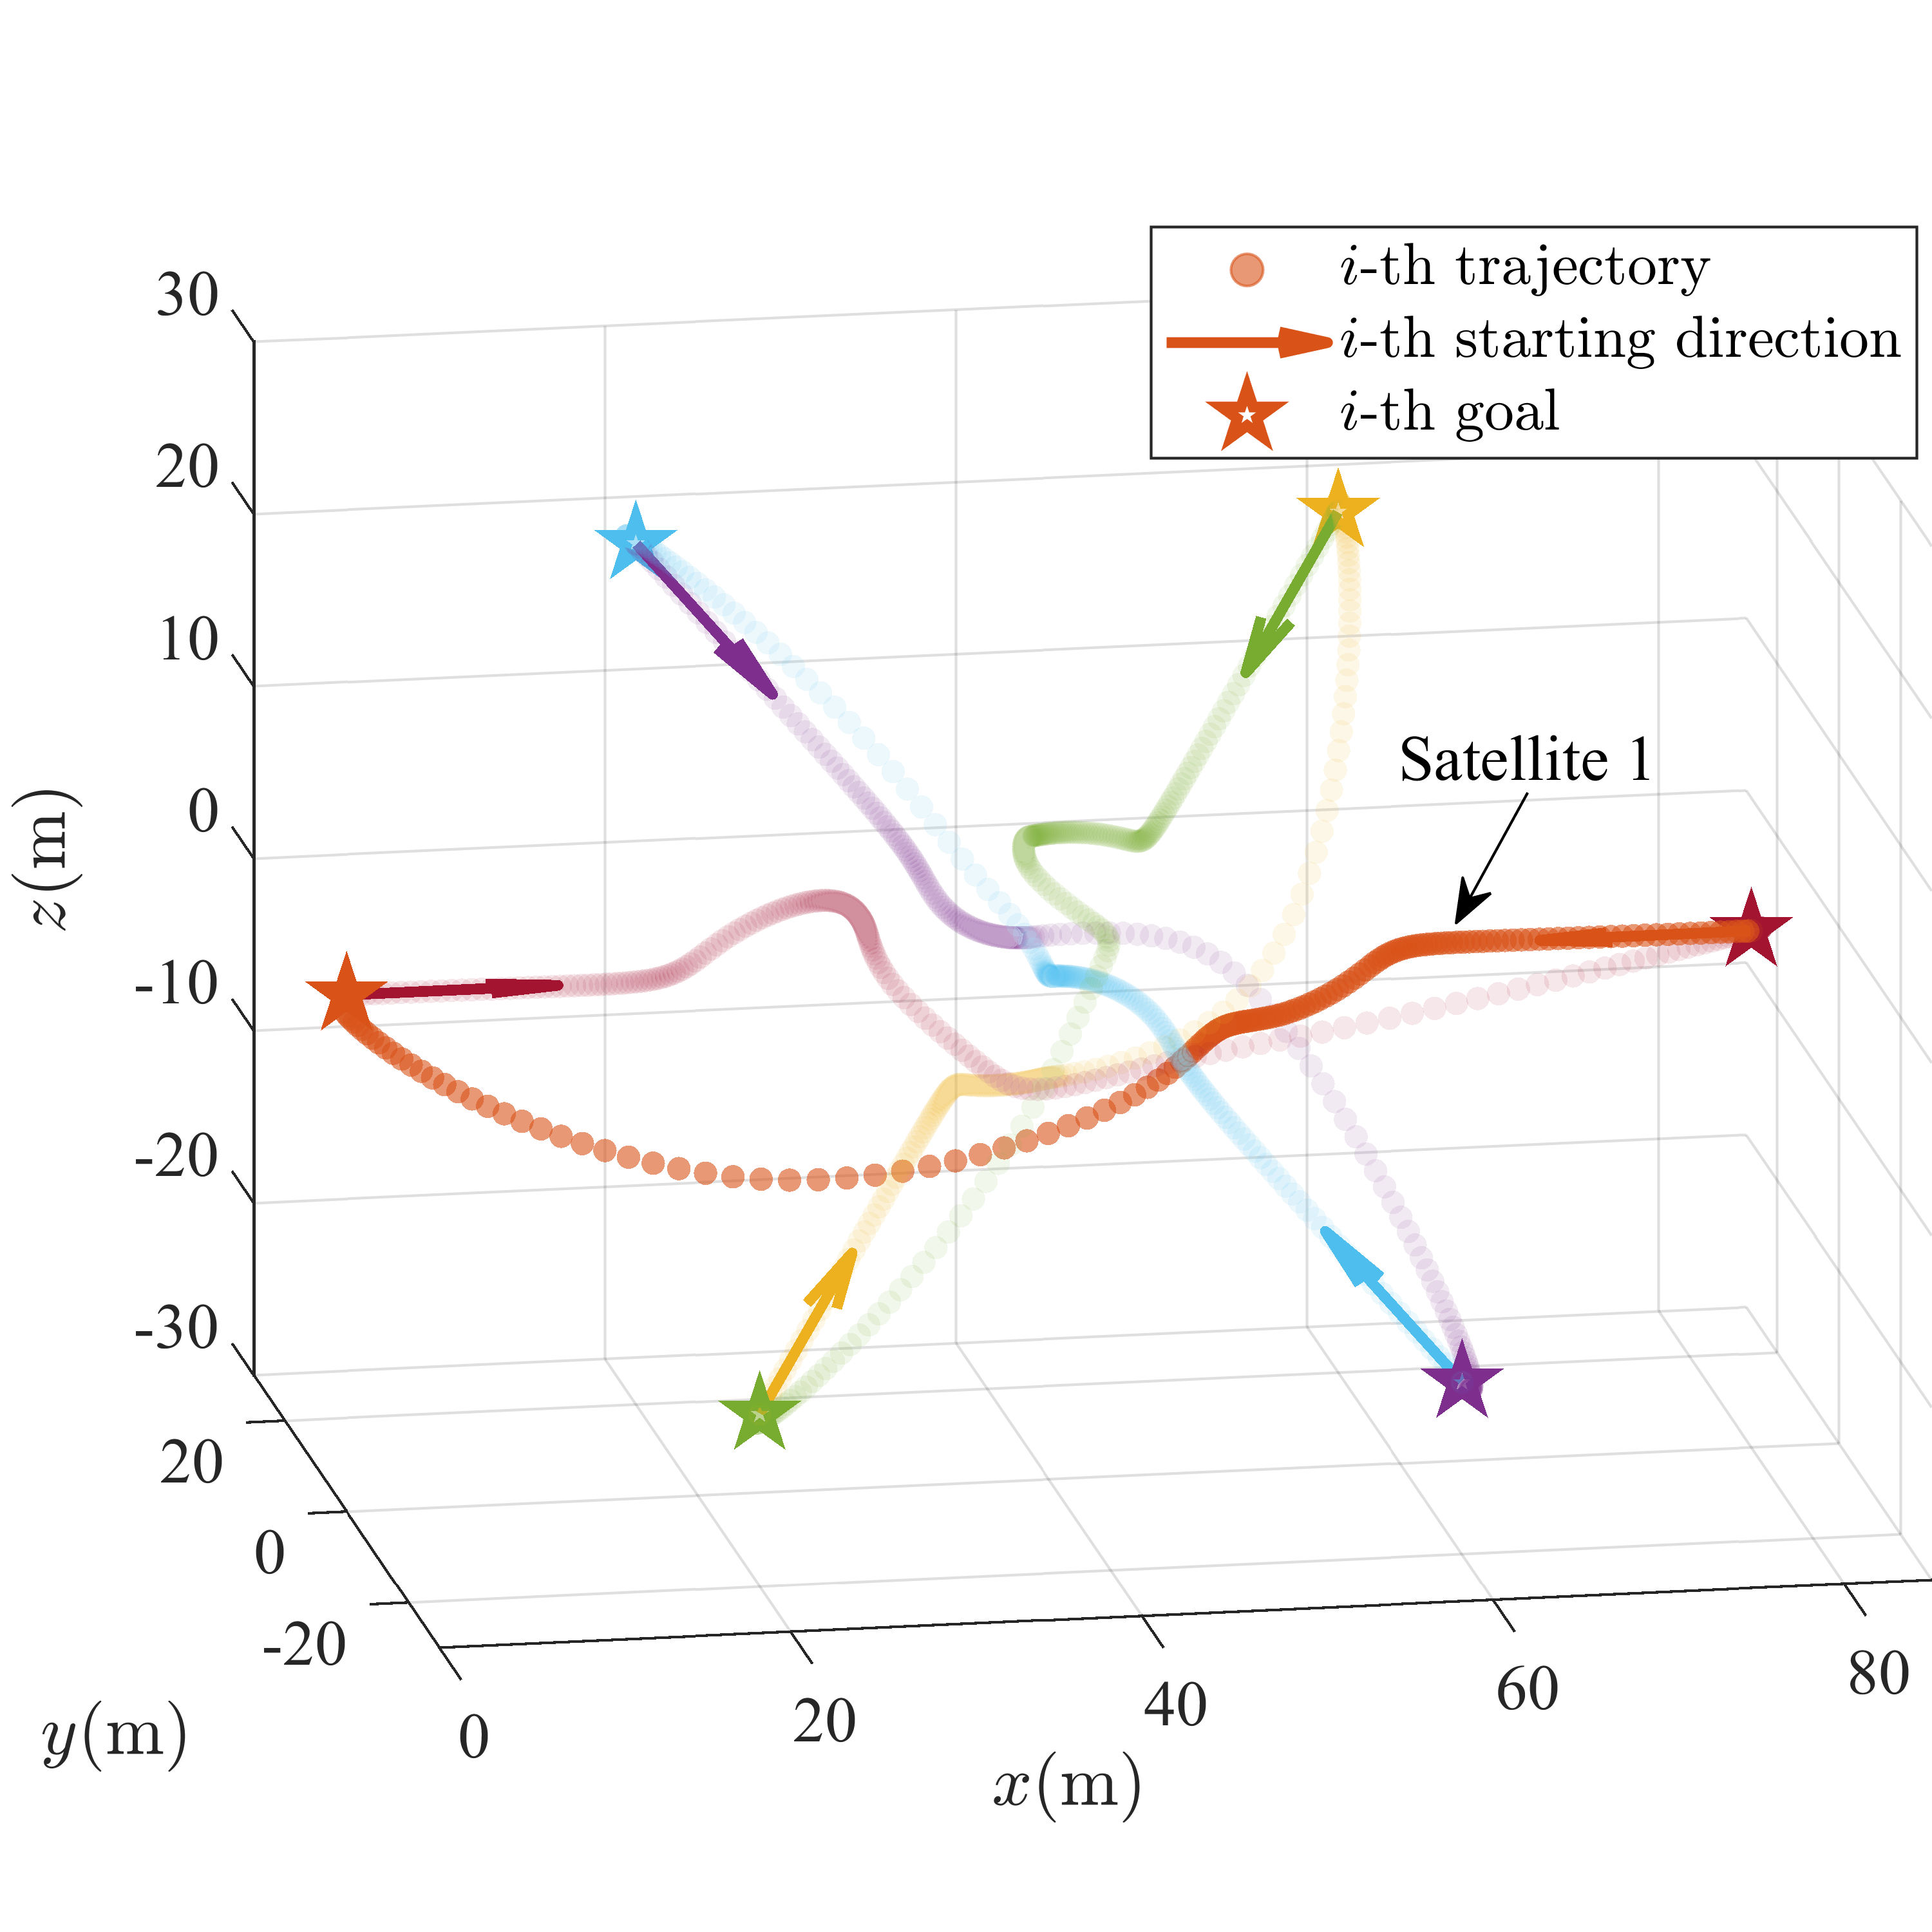
\includegraphics[width=0.9\linewidth, trim = \leftClip{} \lowerClip{} \rightClip{} \upperClip{}, clip]{llm2.png} \label{fig:llm2} } \\
   \subfloat[$T_1 = 321.5\mathrm{s}$]{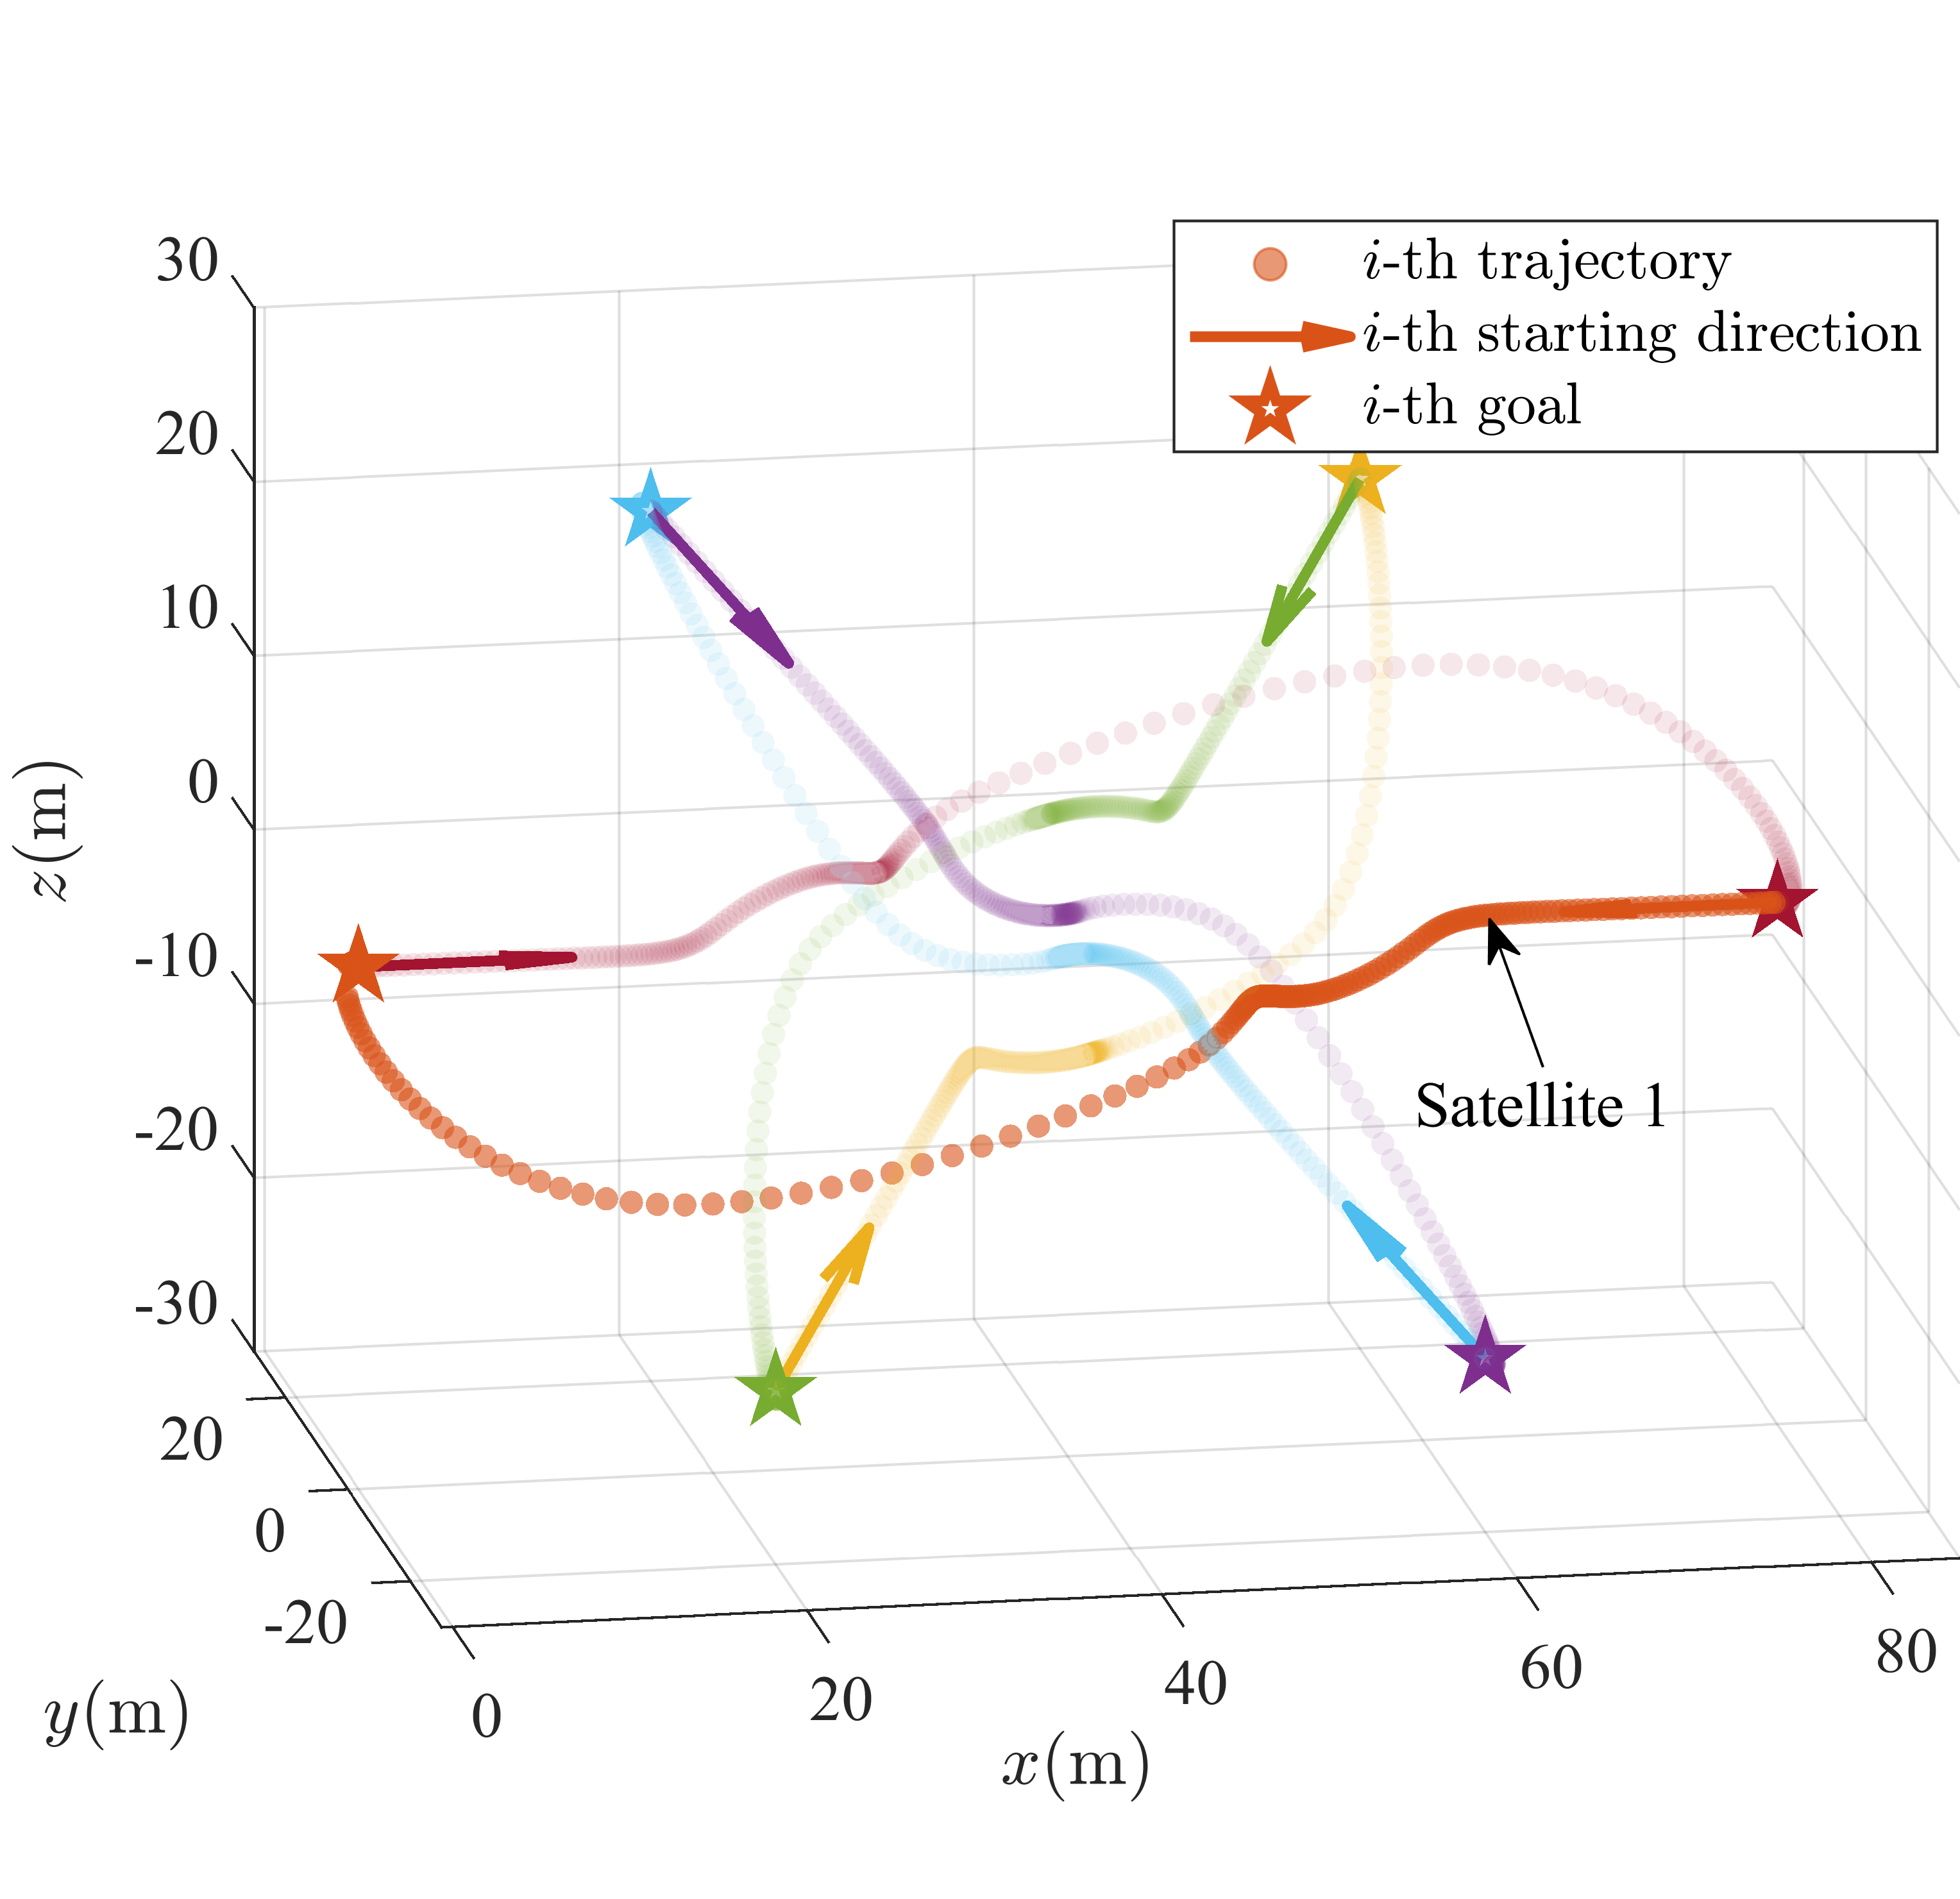
\includegraphics[width=0.9\linewidth, trim = \leftClip{} \lowerClip{} \rightClip{} \upperClip{}, clip]{llm3.png} \label{fig:llm3} } 
   \caption{Swarm behavior with different LLM prompts.}
   \label{fig:llmexp}
\end{figure}

% \section{Conclusion}

% A conclusion section is not required. Although a conclusion may review
% the main points of the paper, do not replicate the abstract as the
% conclusion. A conclusion might elaborate on the importance of the work
% or suggest applications and extensions.

% \begin{ack}
% Place acknowledgments here.
% \end{ack}

\bibliography{ref_noDOI}             % bib file to produce the bibliography
                                                     % with bibtex (preferred)

\end{document}
